%!TEX root = thesis.tex
\immediate\write18{makeglossaries -q "\jobname"}

%:-------------------------- Preamble -----------------------

% Three languages are supported, which will be reflected in the logo on the front page. Pass the appropriate language
% specified as a class option to uit-thesis. Passing any other languages supported by babel will result in the default
% language on the frontpage. If no language is passed, the default is selected.
%  - USenglish (default)
%  - norsk
%  - samin
% The frontpage comes in two variants, Master's thesis and PhD. Master is default, use classoption 'phd' for the PhD version.
\documentclass[USenglish]{uit-thesis}


% Lorem ipsum
%\usepackage{lipsum}


\usepackage{listings-golang} % import this package after listings
\usepackage{color}

\lstset{ % add your own preferences
    frame=single,
    basicstyle=\footnotesize\ttfamily,
    keywordstyle=\color{purple}\ttfamily,
    commentstyle=\color{blue},
    numbers=left,
    numbersep=5pt,
    showstringspaces=false, 
    stringstyle=\color{blue},
    tabsize=4,
    language=Golang % this is it !
}

\makeglossaries

% Add external glossaryentries
\loadglsentries{acronyms}
\newacronym{api}{API}{application programming interface}\glsunset{api}
\newacronym{2api}{2API}{application programming interface}
\newacronym{d3}{D3}{Data-Driven Documents}
\newacronym{html5}{HTML5}{version 5 of the HyperText Markup Language standard}
\newacronym{wsn}{WSN}{Wireless Sensor Network}
\newacronym{bs}{BS}{Base Station}
\newacronym{ch}{CH}{Cluster Head}
\newacronym{coat}{COAT}{Climate-ecological Observatory for Arctic Tundra}
\newacronym{ou}{OU}{Observation Unit}
\newacronym{leach}{LEACH}{Low-Energy Adaptive Clustering Hierarchy}
\newacronym{fleach}{F-LEACH}{Fuzzy-LEACH}
\newacronym{gbcp}{GBCP}{Gossip-based communication protocol}
\newacronym{pegasis}{PEGASIS}{Power-efficient gathering in sensor information systems}
\newacronym{gaf}{GAF}{Geographic Adaptive Fidelity}
\newacronym{gear}{GEAR}{Geographic and Energy-Aware Routing}
\newacronym{tcp}{TCP}{Transmission Control Protocol}
\newacronym{p2p}{P2P}{Peer-To-Peer}
\newacronym{dao}{DAO}{Distributed Arctic Observation}


\newglossaryentry{thesis}
{
  name=thesis,
  description={is a document submitted in support of candidature for an
    academic degree or professional qualification presenting the author's research and findings},
}
\newglossaryentry{lage}
{
  name={long ass glossary entry},
  description={is a long ass entry with a lot of text describing the properties of the glossary entry. Hopefully this spans some lines now.},
}


\newcommand{\listdefinitionname}{My list of definitions}
\newlistof{definition}{def}{\listdefinitionname}
\newcommand{\definition}[1]{%
  \refstepcounter{definition}%
  \par\noindent\textbf{The Definition~\thedefinition. #1}%
  \addcontentsline{def}{definition}
    {\protect\numberline{\thechapter.\thedefinition}#1}\par%
}

\font\zerofont = cmsy7 at 9.3pt

\begin{document}

%:-------------------------- Frontpage ------------------------

\title{Peer Observations of Observation Units}
%\subtitle{Subtitle}			% Optional
\author{Camilla Stormoen}
\thesisfaculty{Faculty of Science and Technology \\ Department of Computer Science}
\thesisprogramme{INF-3981 Master's Thesis in Computer Science ... May 2018}
%\ThesisFrontpageImage{example_image.jpg}	% Optional


\maketitle

%:-------------------------- Frontmatter -----------------------
\frontmatter

%\begin{dedication}
%To Leslie.
%Fuck you very much.
%\end{dedication}


%\begin{epigraph}
%\epigraphitem{Simplicity is prerequisite for reliability.}{Edsger Dijkstra}
%\epigraphitem{Beware of bugs in the above code;\\I have only proved it correct, not tried it.}{Donald Knuth}
%\end{epigraph}


\begin{abstract}
\glsresetall
%What is wrong with the world? Motivation 1-3 sentences, Arch, Des, Imp, Exp 1,2-3 sentences, results and main conclusion.

The Arctic Tundra in the far northern hemisphere is one of ecosystems that are most affected by the climate changes in the world today. Five Fram Center\footnote{\url{http://www.framsenteret.no/english}} institutions developed a long-term research project called \gls{coat}. Their goal is to create robust observation systems which enable documentation and understanding of climate change impacts on the Arctic tundra ecosystems.


This thesis describes a prototype of a Wireless Sensor Network (\gls{wsn}) system where nodes in the network creates clusters of Observation Units (\glspl{ou}) to accumulate data. The purpose is to fetch and accumulate data observed by \gls{ou}s for further use and to provide for a more flexible and powerful sensor in the \gls{coat} monitoring of the Arctic Tundra.

We describe a system where nodes discover each other through a broadcast range. Together they form clusters. Each cluster elect a Cluster Head (\gls{ch}) which is responsible for sending out a request for gather and accumulate data from the other nodes in the cluster. The \glspl{ch} are rotating to save battery.


\textbf{HIGH/LOW etc... siste del uklart..}

Results show that the system have a stable CPU and memory usage during execution. Experiments also show that the number of receiving packets at \glspl{ch} is lower than sent packets which indicates that the nodes in the system accumulates data when intended.

Main conclusion/insight..

\end{abstract}


\begin{acknowledgement}
First I would like to thank my main advisor Professor Otto Anshus and co-advisor Professor John Markus Bjørndalen for providing guidance, support, ideas and feedback whenever I needed it through this thesis.

I would also like to thank TK and the administration...

I want to express my sincerest gratitude to the \textit{Masterinos}. I would not have made it without you guys. 

I would also like to thanks my parents for encouraging me to take a higher education and supporting me through every decision. At last I would like to thank my boyfriend.

\end{acknowledgement}

\tableofcontents

%\listofdefinition

\listoflistings


\printacronyms


%:-------------------------- Mainmatter -----------------------
\mainmatter

\chapter{Introduction}
\glsresetall
The Arctic tundra in the far northern hemisphere is challenged by climate changes in the world today and is one of the ecosystems that are most affected by these changes \cite{coat2016}. Five Fram Center\footnote{\url{http://www.framsenteret.no/english}} institutions developed a long-term research project called \gls{coat}. Their goal is to create robust observation systems which enable documentation and understanding of climate change impacts on the Arctic tundra ecosystems. COAT was in autumn 2015 granted substantial funding to establish research infrastructure which allowed them to start up a research infrastructure during 2016-2020 \cite{coat2016}.

\gls{wsn} is a system that consists of hundreds or thousands of low-cost micro-sensor nodes. These nodes monitor and collect physical and environmental conditions. The various activities  in the sensor nodes consume lots of energy and the battery of the sensor node is difficult to recharge in wireless scenarios and also because the sensor nodes are located at remote areas in the Arctic tundra.


%It is beneficial to make these sensors as cheap and energy-efficient as possible.

This thesis presents the architecture, design, implementation and evaluation of a peer observation system that can observe and accumulate data from other peers in multiple clusters in a network.


\section{Motivation}
The motivation behind this project is that multiple \gls{dao}-Stores \cite{dao} may want different data from sensors deployed in the Arctic Tundra. With all the data gathered from each sensor, will there be a need for gathering data that is most important for each \gls{dao}-Store. One example can be a \gls{dao}-Store \gls{coat} that wants data such as images for their research.

This dissertation will develop an approach to let \gls{ou} observe each other and gradually accumulate data to \glspl{ou} being a \gls{dao}-Store. There can be multiple \glspl{dao}-Stores depending on user needs. The purpose is to fetch and accumulate data observed by \gls{ou}s for further use and to provide for a more flexible and powerful sensor in the \gls{coat} monitoring of the Arctic Tundra.


%This project will develop an approach to 
%\begin{itemize}
%\item Let observation units observe data observed by observation units. 
%\item To gradually accumulate the data to observation units being a DAO Store (there can be multiple DAO Stores depending on user needs).
%\item Do a prototype of such a system focused on three levels of observation units: (i) In-situ observation units being (ii) observed by back-end observation units, being (iii) observed by a DAO-Store observation unit.
%\end{itemize}


\section{Contributions}
The dissertation makes the following contributions:

\begin{itemize}
\item An description of relevant \gls{wsn}s and routing techniques in \gls{wsn}s.
\item An (architecture, design)/\textbf{description} and implementation of a \gls{wsn} system.
\item An evaluation of the system.
\item Thoughts on further improvements to the current system and future work.
\end{itemize}


%\section{Assumptions}
%Avgrense viktig!

\section{Limitations}
%Avgrense viktig!
%Fokus på cluster som tar hensyn til batteri mtp at nodene er ute i tundraen og ikke har mye tilgang til strøm.. redundancy, reliability, scalability?? 
This dissertation focuses on creating a prototype of a cluster network and do not focus on the data passed between the nodes. Data collected from the nodes are not actual data collected from sensors, as this isn't crucial for the system implementation itself.


\newpage

\section{Outline}
This thesis is structured into X chapters including the introduction.

\begin{description}
\item[Chapter 2] describes different routing- and communication protocols in \gls{wsn}s.
\item[Chapter 3] presents related work in the field of \gls{wsn}, node communication and comparing it to the work done in this thesis.
\item[Chapter 4] describes the technical idea.
\item[Chapter 5] describes the system architecture.
\item[Chapter 6] describes the design of the system and how a cluster network may appear.
\item[Chapter 7] describes the implementation of the system together with choices and issues during implementation.
\item[Chapter 8] describes the experimental setup, metrics used to evaluate the implemented system and the results from the experiments.
\item[Chapter 9] discusses our approach, experiences, how we solved the problem and why we chose the solution we ended up with.
\item[Chapter 10] concludes the thesis.
\item[Chapter 11] suggests future work to improve the system.
\item[Chapter 12] Appendix
\end{description}


%\subsection{A subsection}
%We can use the \ac{api} to \ac{2api} do stuff, and write about what we did in a \gls{thesis}!

%This is some stuff, {\sc smallcaps {\em smallcapsemphasized}} {\em regularemphasized}

%\Gls{lage}: a test glossary entry.

%If the acronym \ac{uit} is displayed, then loadglsentries works.

%It is fun to use modern \upsc{OpenMP} technology!\footnote{This is a snarky footnote. Words and etc. Semantic web technologies are technologies that enable semantification of the Web as we know it today. Hopefully this spans some lines now.}

%It is fun to use \emph{modern \upsc{OpenMP}} technology! And it is fun to use \ac{d3} and \ac{html5}.

%\definition{Some other definition}



\chapter{Routing Techniques in WSNs}
\glsresetall
\gls{wsn} is a system that consists of hundreds or thousands of low-cost micro-sensor nodes which monitor and collect physical and environmental conditions. Figure \ref{fig:wsn} shows how a \gls{wsn} architecture can be, with multi-hop routing. 

%\definition{Multi-hop routing is a type of communication in radio networks where nodes use other nodes as relays to reach some destination.}

\gls{wsn}s  main task is to periodically collect information of the interested area and broadcast the information to a \gls{bs}. An easy approach to achieve this task is to make each sensor node transmit their data directly to the BS. But the problem is that the \gls{bs} can be far away from the sensor node so a direct data transmission would not be possible, or if the routing path from the sensor node to the \gls{bs} is long, the sensor node may require more energy than available. There are multiple hierarchical protocols that has been proposed as a solution to this problem.

\begin{figure} [!ht]
\centering
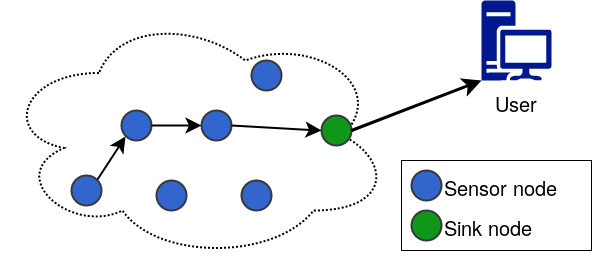
\includegraphics[width=\textwidth]{wsn.png}
\caption{Figure shows an example of a multi-hop \gls{wsn} architecture.}
\label{fig:wsn}
\end{figure}

%\newpage

\section{Routing Protocols in WSNs}
\subsection{Hierarchical Routing}
Hierarchical routing, also called cluster-based routing, is a well know technique for network routing with special advantages related to scalability, efficient communication and lower energy consumption in WSNs. Each cluster in the hierarchical routing protocol have a special node which is responsible for coordinating data transmission between all nodes in the cluster \cite{leach, leach_perf, routing_survey}.

%\textit{Hierarchical routing is an efficient way to lower energy consumption within a cluster, performing data aggregation and fusion in order to decrease the number of transmitted messages to the \gls{bs}.}

Two approaches based on hierarchical routing are \gls{leach}\cite{leach} and \gls{pegasis}\cite{pegasis} which are described in Chapter \ref{chap:related_work}.


\subsection{Location-based Routing}
In location-based routing, nodes are addressed based on their location. The distance between a node and its neighbour can be estimated by incoming signal strengths, by GPS or via coordination among nodes \cite{routing_survey}. Two approaches are \gls{gaf}\cite{gaf} and \gls{gear}\cite{gear}.


\section{Flood And Gossiping Protocol}
\subsection{Flooding Protocol}
The simplest forwarding rule is to flood the network. In flooding, a node sends a packet received to all its neighbours expept the neighbours which sent the packet until the packet arrives at the destination or maximum number of hops for the packet is reached. Its biggest drawback is thatyhe protocol is not an energy efficient protocol and is not designed for sensor networks \cite{wsnbook}.

\subsection{Gossiping Protocol}
Gossiping is a modified version of flooding attempting to correct some of its drawbacks. In gossiping, a node with updated data will contact an arbitrary node with updated information. However, it is possible that the contacted node was updated by another node and in that case may not spreading the update any further \cite{dsbook}.


\chapter{Related Work} \label{chap:related_work}
\glsresetall
%\section{Routing Protocols in WSNs}
To improve the overall energy dissipaton of \gls{wsn}s, \gls{leach} \cite{leach} introduce a hierarchical clustering algorithm for sensor networks. It is self-organized and use randomization to distribute the energy load evenly among the sensors in the network. The sensor nodes organize themselves into local clusters where one node is the local \gls{bs} or \gls{ch}. The \gls{ch} are not fixed to avoid nodes to drain their battery and to spread the energy usage over multiple nodes. The nodes self-elect a new \gls{ch} depending on the amount of energy left at the nodes at different time-intervals. \gls{leach} is divided into different rounds where each round include a setup phase and a steady-state phase \cite{tree_based}. In the setup phase will each node decide whether to become a \gls{ch} or not. When a \gls{ch} is chosen, each node will select its own \gls{ch} based on the distance between the node and the \gls{ch} and join the cluster. In the steady-state phase will the \gls{ch} fuse the received data from the node members in the cluster and send it to \gls{bs}. Details of the \gls{leach} algorithm is listed below:

\begin{itemize}
\item \textbf{Advertisement Phase:} where each node decides whether to become a \gls{ch} or not. If a node has elected itself as \gls{ch}, it will broadcast a message to the rest of the nodes. Each node will then decide which cluster it belongs to for this round.
\item \textbf{Cluster Set-Up Phase:} the nodes will inform the \gls{ch} that it will be a member of the cluster.
\item \textbf{Schedule Phase:} based on the number of nodes in the cluster, the \gls{ch} creates a schedule telling each node when it can transmit data.
\item \textbf{Data Transmission:} as long as a node has data, it sends data to the \gls{ch} during their allocated transmission time. After a certain time, the next round begins with each node determine if it should be a \gls{ch}. 
\end{itemize}

In contrast, will nodes in our approach first connect to a cluster and then start a \gls{ch} election rather than elect a \gls{ch} first and then nodes joining the cluster. %This is described further in Section/Chapter \ref{xx}.
A resemblance between the two approaches is that neither of them consider a node's energy level when calculating the \gls{ch}. Details of our approach is listed below:

\begin{itemize}
\item \textbf{Cluster Set-up Phase:} nodes will create clusters by connecting to reachable nodes.
\item \textbf{Advertisement Phase:} when a node joins a cluster, it will start a \gls{ch} election to decide whether to become a \gls{ch} or not. The nodes will gossip the election until the \gls{ch} is consistent at all nodes.
\item \textbf{Data Transmission:} the \gls{ch} broadcasts a message to all nodes in the cluster asking for data. The \gls{ch} will ask for data a random number of times and when it has received all the data, the next round of a \gls{ch} election begins.
\end{itemize}

%\begin{equation}
%T(n) = \frac{P}{1-P\times(r \bmod \frac{1}{P})}
%\end{equation}

%\begin{equation} \label{eq:leach}
%T(n) = \begin{cases}\frac{P}{1-P\times(r \bmod \frac{1}{P})} & if n \in G
%\\0 & otherwise\end{cases}
%\end{equation}


\gls{leach} do not consider a node's energy level when calculating the \gls{ch}. It has therefore been a benchmark for improving algorithms such as the centralized clustering algorithm LEACH-C \cite {leach_c} and distributed clustering algorithm such as LEACH-E \cite{leach_e} and LEACH-B \cite{leach_b}. They concentrate on energy consumption reducing a nodes residual energy and more relevant criterions \cite{dec_cb_alg}.


%\begin{equation} \label{leach_c}
%P_{i}(t)=\min\left\{\frac{E_{i}(t)}{E_{total}(t)}k, 1\right\}
%\end{equation}

\Gls{fleach} \cite{fuzzy_logic, ch_fuzzy} have three different fuzzy descriptors such as energy, concentration and centrality used to complement the cluster head selection process. The \gls{bs} performs the \gls{ch} election in each round by computing the chances of a node becoming a \gls{ch} by calculating the three fuzzy descriptors. \Gls{fleach} also assumes that the \gls{bs} elects the appropriate \gls{ch} because it has a complete information about the whole network.

In contrast to \gls{fleach}, our approach will elect a \gls{ch} by the nodes in the cluster and not in a \gls{bs}. The \gls{ch} election will not consider sub-factors such as battery level or number of nodes in the cluster.


\gls{gaf} \cite{gaf} propose a energy-aware location-based routing algorithm designed for mobile ad hoc networks, but are also applicable for sensor networks. First, the network area is divided into different zones and forms virtual grids. Inside each zone, the nodes communicate with each other to to figure out their different roles. E.g., one node will be elected to stay awake for a certain period of time and is responsible for monitoring and reporting data to the \gls{bs} while the rest of the nodes goes to sleep. Each node is also located by a GPS-position which is associated with a point in the virtual grid. Nodes within the same point are considered equivalent in terms of packet routing. This means that some nodes within the same point can sleep in order to save energy. This apporach is also an example of adaptive fidelity \cite{adfidelity} where the quality (fidelity) of the answer of the algorithm can be traded against battery lifetime, network bandwidth, or number of active sensors.

Our approach have no adaptive fidelity algorithm for trading battery lifetime, network bandwidth or number of active sensors. However, our approach use simulated GPS-coordinates (x,y) to place nodes within a grid as similar to \gls{gaf}. Nodes can only contact other nodes within a simulated broadcast width. This is explained further in Section \ref{chap:implementation}. In contrast to \gls{gaf}, will \gls{ch} and regular nodes in our approach accumulate received data  with its own data.


\Gls{pegasis} is a chain-based protocol with the idea to form a chain among the sensor nodes so each node will receive and transmit data to a close neighbour. The sensor nodes will also take turns on being the leader for transmitting data to the \gls{bs} and therefore distribute the energy load evenly among the sensor nodes. The chain can be organized by the nodes themselves using a greedy algorithm starting from some node, or the \gls{bs} can compute the chain and broadcast it to all the nodes in the network \cite{pegasis}. The greedy algorithm assumes that all nodes have a global knowledge of the network for constructing the chain. Each node, except the end nodes, performs data aggregation with data received from its neighbours data and transmit that to its other neighbours.

Our approach do not assume that all nodes have a global knowledge of the network and computing the path is done in the same task as electing a \gls{ch}. Furthermore, our approach is a cluster based protocol and not a greedy based approach used for chain formation. Our network have one \gls{ch} per cluster instead of only one node who will aggregate data and pass it to the \gls{bs}.


To increase the robustness of devices and lower power consumptions, ZebraNet \cite{zebranet} provides a low-power wireless system for position tracking of wildlife by using peer-to-peer network techniques. This reduces the researchers effort to manage the sensors and collecting logged data for their research. The radios on their devices also operates on different frequencies and have different bandwidth, range and other characteristics.

A diversity to our approach is that ZebraNet stores multiple copies of the same data across multiple nodes while our approach forwards the data to the next node in the path to leader. They've also deployed their sensors on zebras in a real-life environment. For us, it's not feasible to deploy sensors out in the real-life Arctic Tundra in such an early development.


%\section{Gossip-based Protocols}
Gossip-based protocols, or epidemic protocols, are popular protocols due to their ability to reliably pass information among a large set on interconnected nodes. Jelasity et al. \cite{gbsampling} provide a \gls{gbcp} where each node have peers to gossip with in a large-scale distributed system \cite{demers}. These nodes can quickly join and leave the network at any given point of time. The general principle of their framework is that every node (1) maintains a relatively small local membership table that provides a partial view of all nodes and (2) periodically refreshes the table using a gossiping procedure.

The difference between \gls{gbcp} and our approach is that our approach does not use a gossip protocol to update its table of nodes, but instead relies on the communication with other nodes to know about the election of a new \gls{ch}, which of the node is the \gls{ch} and when a node should accumulate data and send it to the \gls{ch}.


%\section{Data Collection/Aggregation in WSNs}
%Di Franscesco et. al. \cite{dataColl}
%Data aggregation is an essential operation in \gls{wsn}s and has emerged as a basic approach in order to reduce the number of transmissions of sensor nodes \cite{dataAgg}.



\chapter{Idea} \label{chap:idea}
\glsresetall
%Technical idea

%Unstructured p2p network..
%Multi-hop communication (not single-hop)

%(Unstructured peer-to-peer networks do not impose a particular structure on the overlay network by design, but rather are formed by nodes that randomly form connections to each other. (Gnutella, Gossip, and Kazaa are examples of unstructured P2P protocols), the role of all peers in the network is the same, unstructured networks are highly robust in the face of high rates of "churn"—that is, when large numbers of peers are frequently joining and leaving the network

%Decentralized- no single point of failure. but coordinators can crash..
%Centralized - Partially centralized: supernodes act as local central indexes, some nodes assume a more important role

%hva er veien, ikke hvilken vei..

The technical idea behind the system is that it should be a partially centralized unstructured \gls{p2p} system where nodes, also called \gls{ou}s, connect to nearby nodes and create clusters. Using an unstructured network would be efficient with regards to a large number of nodes that are frequently joining and leaving the network since it's highly low cost in the face of high rates of churn. The technical idea is shown in Figure \ref{fig:idea}. 

\begin{figure}
\centering
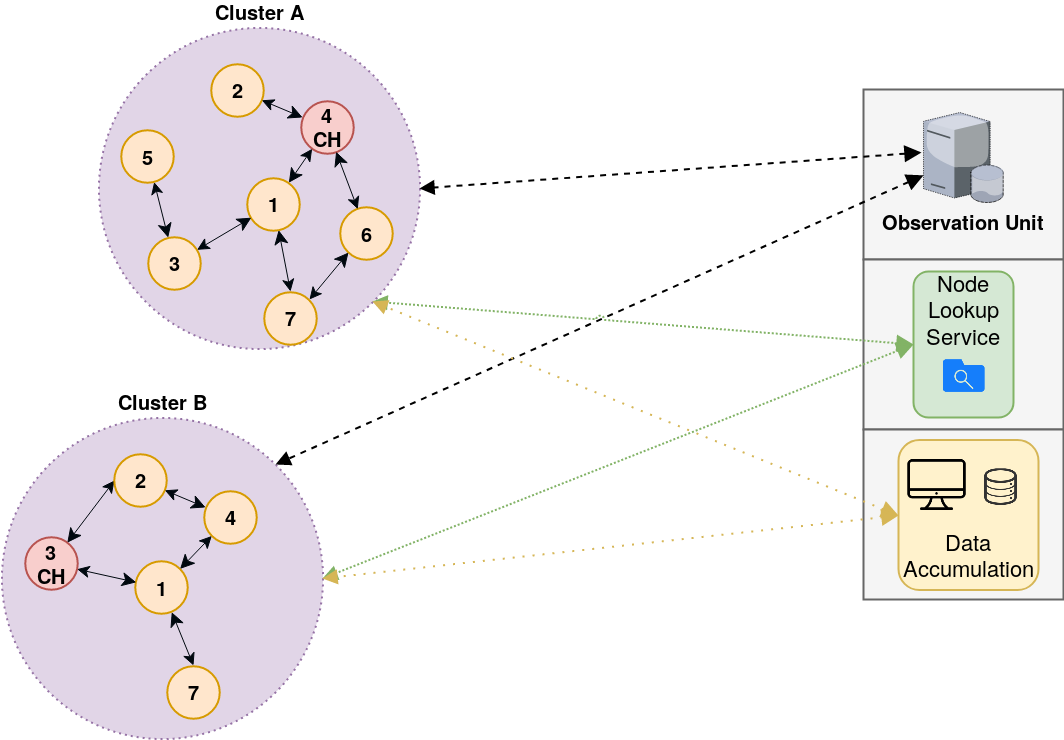
\includegraphics[width=\textwidth]{idea.png}
\caption{Figure shows the technical idea of the system.}
\label{fig:idea}
\end{figure}


The node lookup service in Figure \ref{fig:idea} should provide a functionality for nodes to discover nearby nodes they can connect to. Together, the nodes creates a network of nodes. However, it may occur that the network will be partitioned into multiple clusters due to nodes not reaching each other.

In a partially centralized network, the role of all peers are the same except of some nodes that assume a more important role. These nodes are called \gls{ch}s or super nodes. These \gls{ch}s will be important when accumulating data for further use. A node will assume a more important role in the network decided by multiple sub-factors. The \gls{ch} nodes are the red nodes in Figure \ref{fig:idea}.

All nodes should be able to observe data observed by other nodes and to gradually accumulate data to \gls{ou}s being a \gls{ch} or e.g. a \gls{dao}-Store.





\chapter{Architecture}
\glsresetall
%Tell it clean/neat. Abstractions, functionalities

This chapter describes the architecture of the system. The main functionality can be divided into 4 sub-sections: a nodes lookup service, discovery of other nodes, data accumulation and incoming- and outgoing network requests. The architecture of the system is presented in Figure \ref{fig:architecture3}.


\begin{figure}
\centering
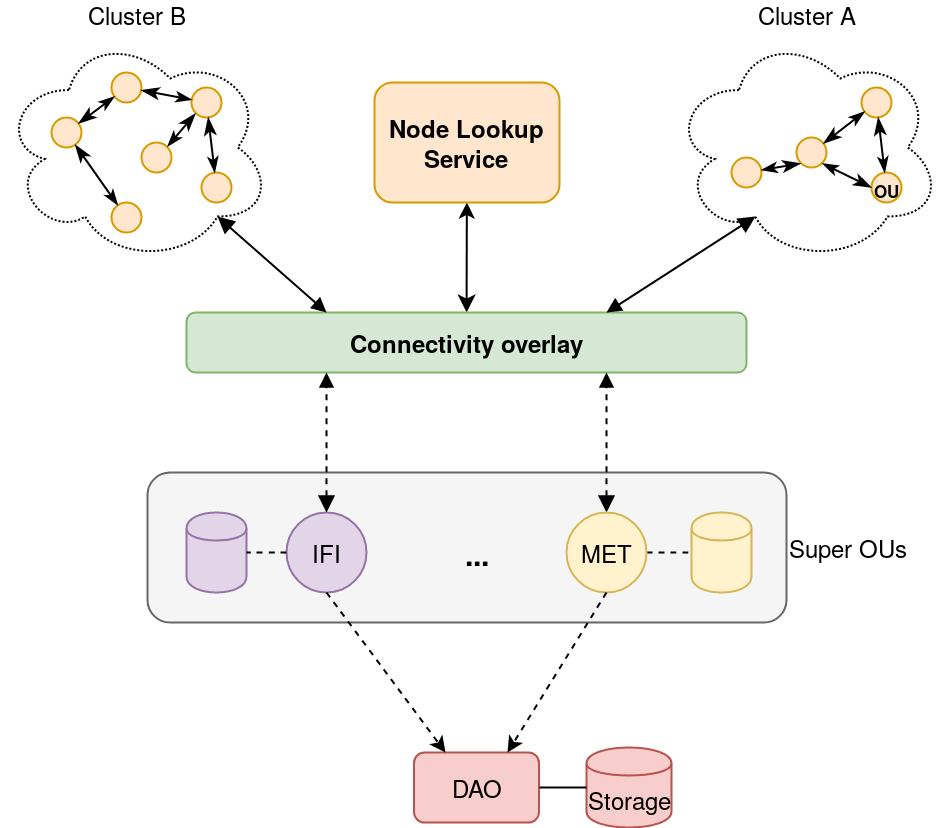
\includegraphics[width=\textwidth]{arch3.png}
\caption{Figure shows the architecture of the system.}
\label{fig:architecture3}
\end{figure}

\section{Node Lookup Service} \label{sec:nodeLS}
The lookup service is responsible for storing all previous discovered nodes and their address. This lookup service is responsible for detecting which nodes that are in range for other nodes and return this result to a corresponding node. 

%Hvordan forlkare at det er en egen service som "simulaerer" range??


\section{Discovery Of Other Nodes} \label{sec:discON}
Each node can only discover other nodes within a simulated radio range. Figure \ref{fig:broadcast_range} shows how a simulated radio range of a node may be discovered. When a new node in the network has been discovered, meta-data about the node such as address be stored locally on the node in the cluster.


\section{Data Accumulation}
A node will accumulate data received from another node if its data hasn't been sent to the \gls{ch}. A \gls{ch} will gather data from nodes in order to provide the accumulated data to a \gls{bs} for further use.


\section{Incoming And Outgoing Network Requests}
A node may receive incoming requests from other nodes in the network. The request handler will handle the request based on the type of request. The types of requests a node may receive are listed below.

\subsection{Connect To Neighbours}
When a node receive a list of neighbours in range from the lookup service, it will try to connect to the neighbours that are within the nodes range. It will only connect to the neighbour node if it receives a OK-message, i.e. the node is allowed to connect.

%\subsubsection{Receive OK From Neighbours}
When a node receives a OK-message it will connect itself to the neighbour. The neighbour will also then be connected to the new node.

\subsection{Cluster Head Election Request}
When a node receives a \gls{ch} election request it will perform a \gls{ch} election and forward the result to it's neigbours which will do a \gls{ch} election as well.
A node may receive a \gls{ch} election request when a node has joined the cluster.

\subsubsection{Cluster Head Election Calculation Request}
If there is a \gls{ch} in the cluster already and a new election should be proposed, a \gls{ch} election calculation request is sent from the leader. Nodes receiving this request will calculate their \gls{ch} election number. %This is explained further in Section xx.

\subsection{Data Transmission}
\subsubsection{Notify Neighbours About Sending Data To Cluster Head}
A node may receive a request that it should send its data to the \gls{ch}. This request is forwarded to the nodes neighbour and so on.

\subsubsection{Send Data To Cluster Head}
This request forwards a nodes data to the next node in the path to the \gls{ch}. If the nodes data receiving this requests isn't sent to the leader of the cluster, will the data be accumulated with the received data and then forwarded to the next node.

%\section{Base Station Access}
%CH should access BS..?


\chapter{Design}
\glsresetall
%Server, p2p, protocols..
In this chapter we will look at the design of the system and present the design of each component. Figure \ref{fig:design} shows how the cluster network may appear in the system. Nodes are connected to other nearby nodes represented by arrows and together they form a cluster network.

\begin{figure}
\centering
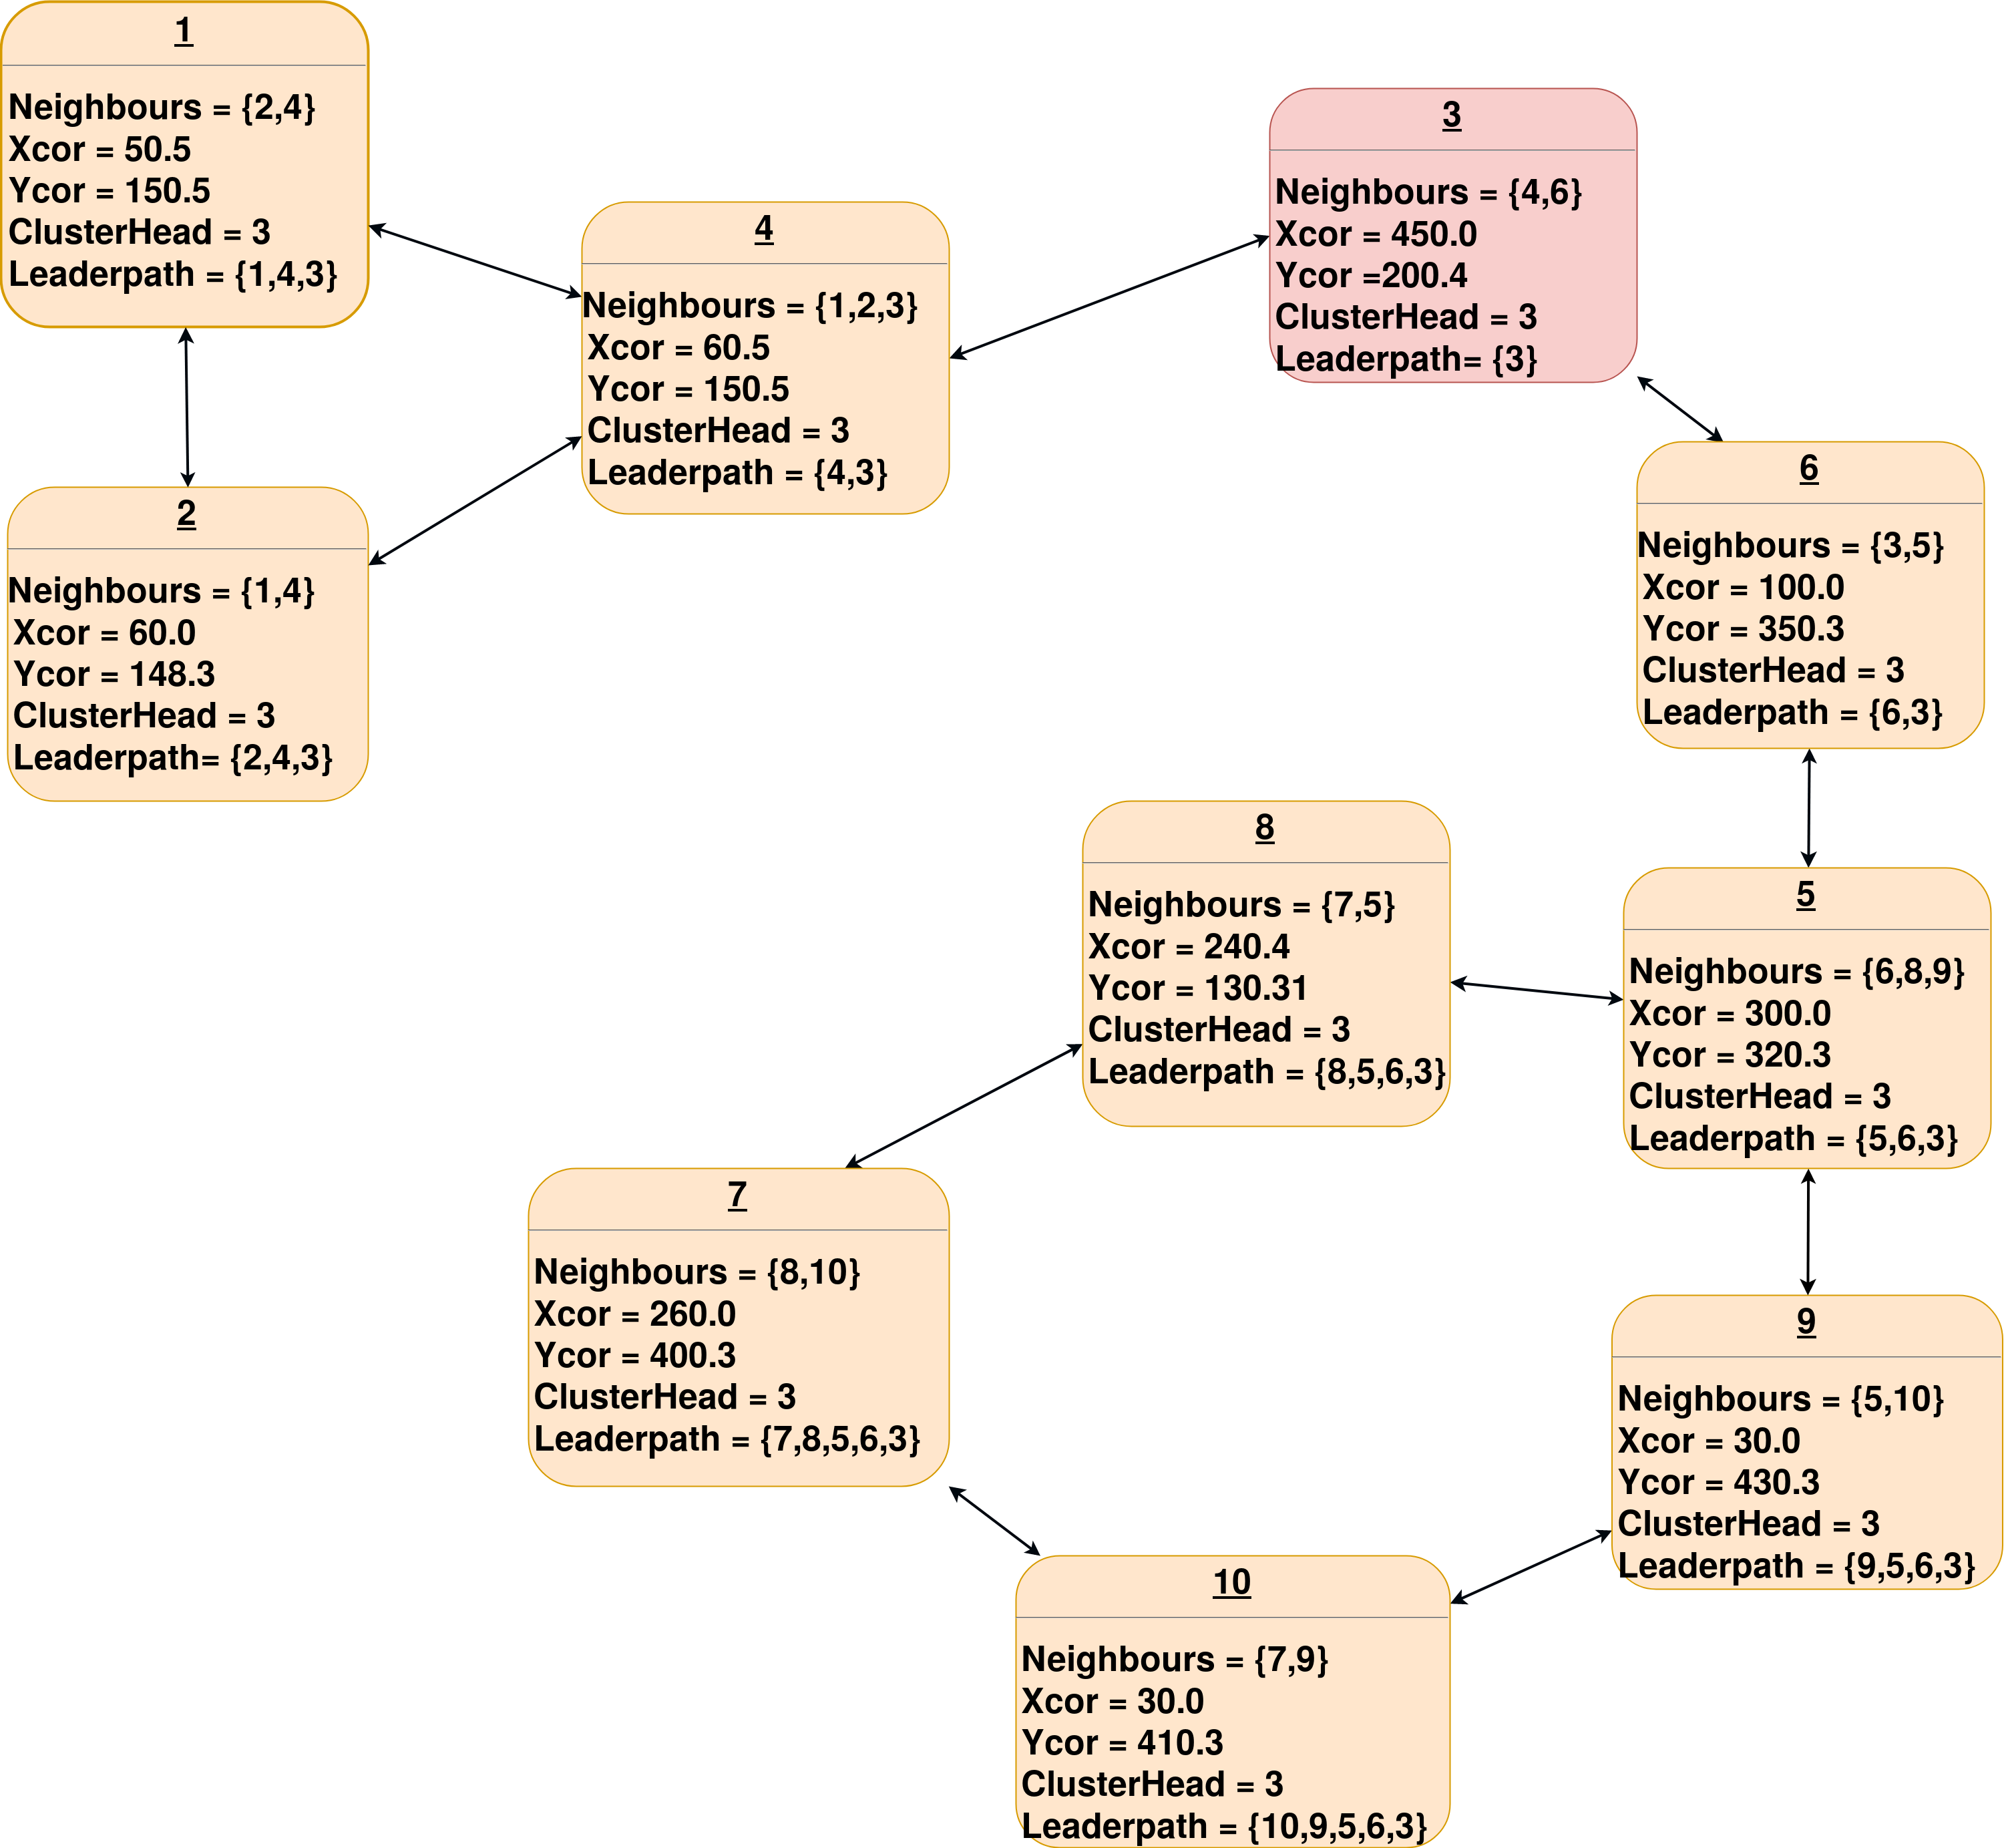
\includegraphics[width=\textwidth]{design.png}
\caption{Figure show design of the system.}
\label{fig:design}
\end{figure}

%\newpage

\section{Discovery Of Other Nodes}
\subsection{Broadcasting}
When a new node start, it will contact the node lookup service to discover other nodes in the network. The node will then initiate a broadcast.
Broadcast is limited due to a radio range limitation where only nodes that are within this range will receive the broadcast, shown in Figure \ref{fig:broadcast_range}. \textit{Node 1} will only reach \textit{node 5} and \textit{node 7}.


\begin{figure}
\centering
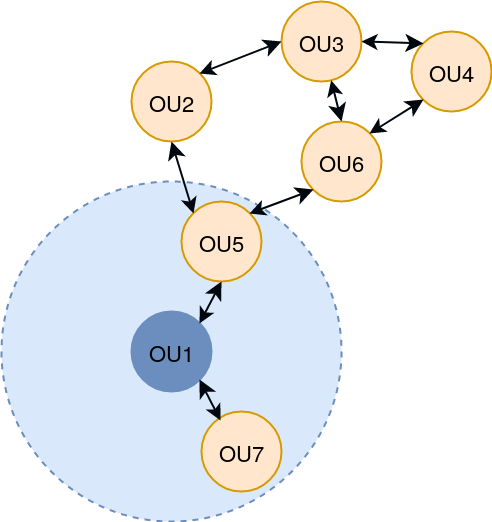
\includegraphics[scale=0.4]{broadcast_range.png}
\caption{Figure show broadcast range of a \gls{ou}.}
\label{fig:broadcast_range}
\end{figure}


%\begin{figure}
%\centering
%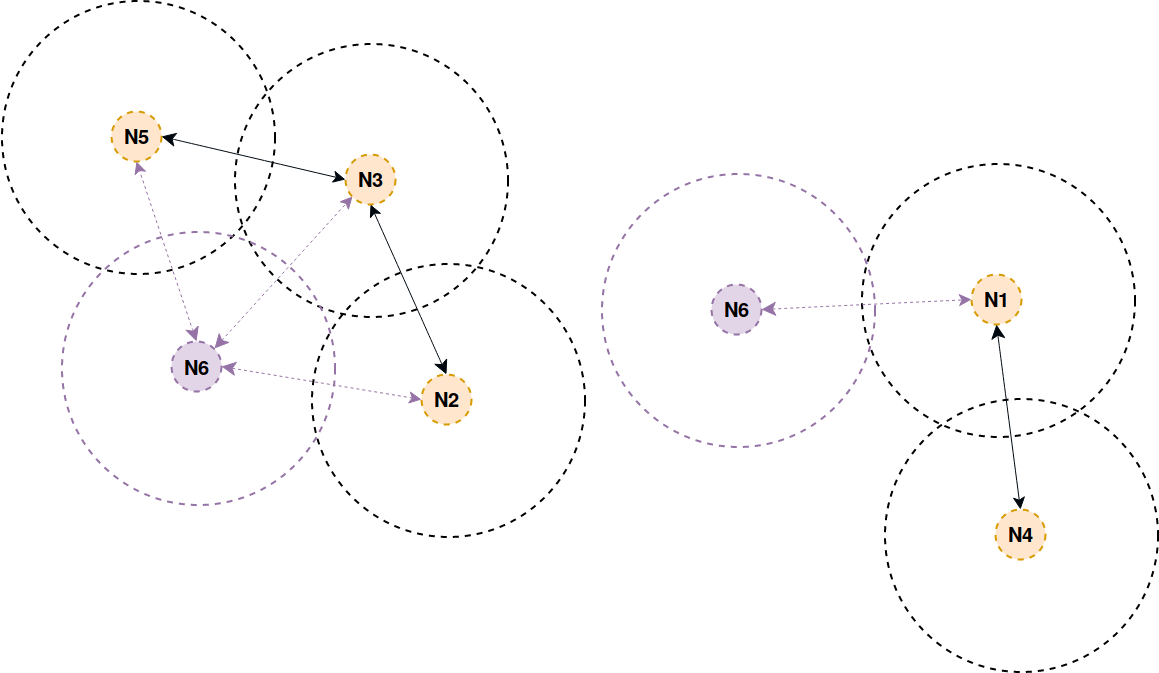
\includegraphics[width=\textwidth]{contactNewNeighbour.png}
%\caption{Figure show how new nodes (purple) contacts their neighbours.}
%\label{fig:contactNeighbour}
%\end{figure}

\newpage

%\section{Maintenance Of Known Nodes}
\section{Cluster Head Election} \label{des:ch_election}
A \gls{ch} election may occur in two scenarios listed below.

%\begin{figure}
%\centering
%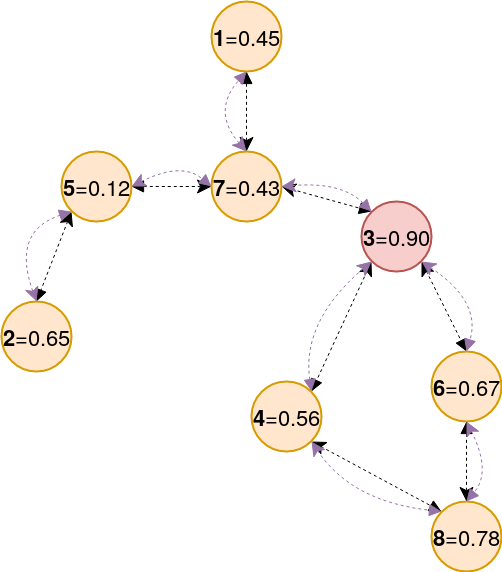
\includegraphics[width=\textwidth]{leaderElection.png}
%\caption{Figure show how a \gls{ch} election is gossiped in the cluster.}
%\label{fig:leaderElection}
%\end{figure}


\subsection{New Node In Cluster Starts Election}
When a new node has joined the cluster, it will start a new \gls{ch} election based on the Bully algorithm. It will calculate it's own \gls{ch}-score and gossip the score to its neighbours. The neighbours will then start a \gls{ch} election comparing the received \gls{ch}-score against their own \gls{ch}-score. The result of the \gls{ch} election will then be gossiped to the node's neighbours with either the received \gls{ch}-score or the nodes own \gls{ch}-score. The gossiped message also contains a path to the \gls{ch}. The node append its own address to the path if the received \gls{ch}-score won the election, otherwise will the path to \gls{ch} only contain the node itself. Eventually a new \gls{ch} is elected by all the nodes and the \gls{ch}-election result will be consistent in the whole cluster. An example of a \gls{ch} election is shown in Figure \ref{fig:newNodeLeaderElection}.

\begin{figure}
\centering
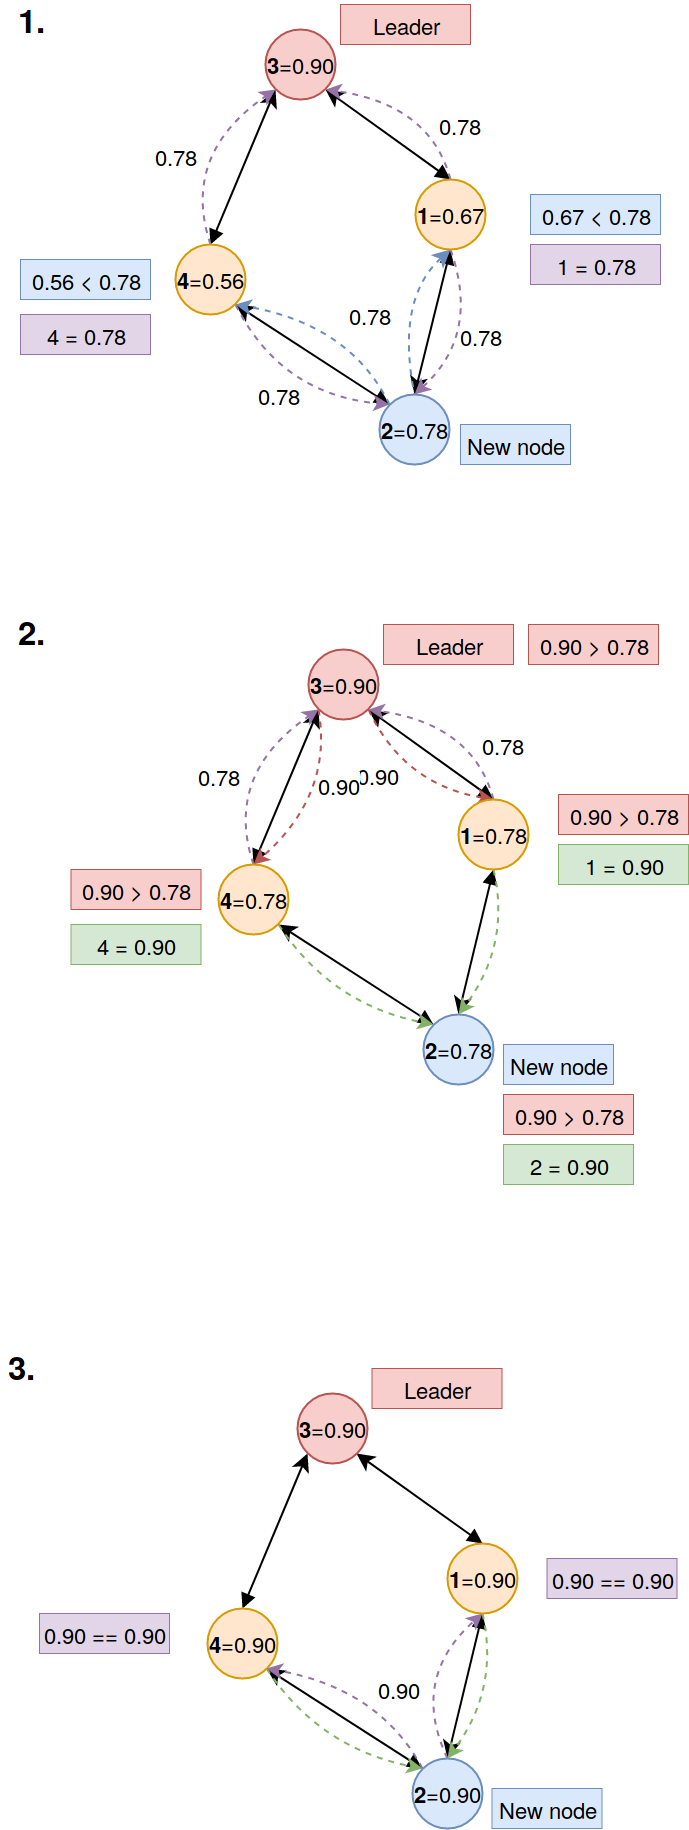
\includegraphics[scale=0.3]{newNodeLeaderElection.png}
\caption{Figure show how a new node starts a \gls{ch} election.}
\label{fig:newNodeLeaderElection}
\end{figure}

\newpage 

\subsection{Cluster Head Starts Election}
When a \gls{ch} has accumulated data 'X' times, it will start a new \gls{ch} election. Initially, the \gls{ch} will gossip a message to nodes the cluster to calculate a new \gls{ch}-score. Then will the \gls{ch} start a new election and gossip this election to the other nodes. The nodes receiving this gossip message will start their leader-election as described in the section above. The election is illustrated in Figure \ref{fig:chWantsLeaderElection}.

\begin{figure}
\centering
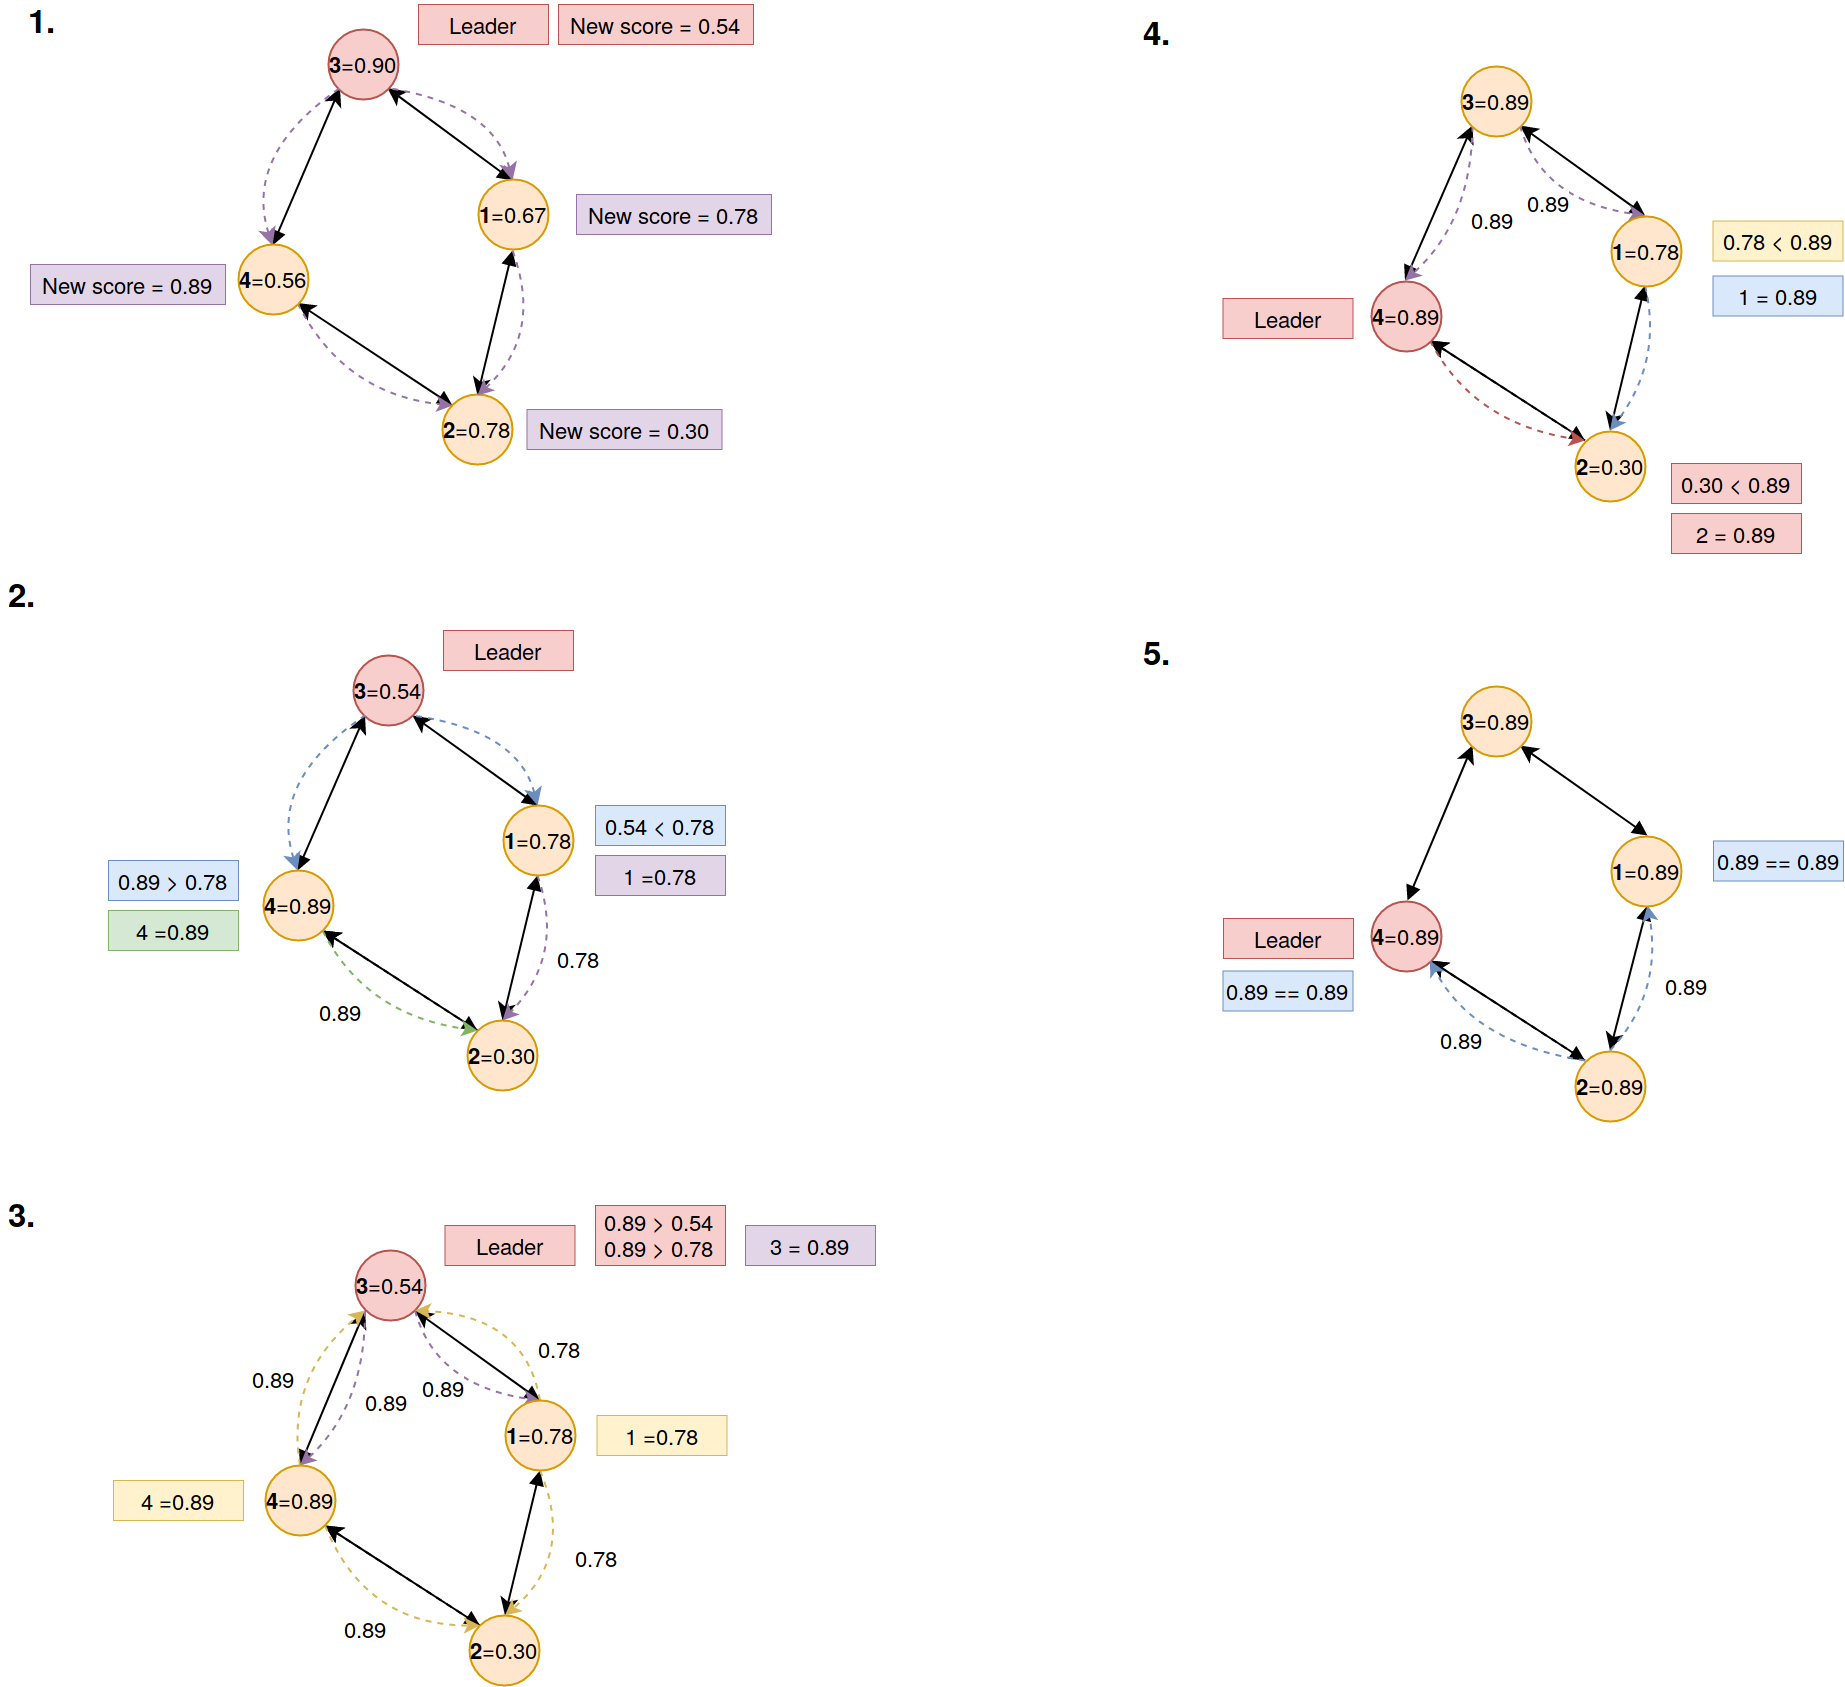
\includegraphics[width=\textwidth]{LeaderNewLeaderElection2.png}
\caption{Figure show how a \gls{ch} starts a \gls{ch} election.}
\label{fig:chWantsLeaderElection}
\end{figure}


\newpage

\section{Data Accumulation}
A \gls{ch} will start gathering data by gossiping a message to nodes in the cluster, illustrated as the red arrows shown in Figure \ref{fig:gaterSendData}. When a node receives this message it will send its data to the next node in the path to the \gls{ch} as Figure \ref{fig:gaterSendData} shows. When a node receive data from another node it will check if it's own data has been sent to the \gls{ch} or not by a fingerprint and a status. If it hasn't been sent earlier, the node will accumulate the received data with its own data, and then send the data to the next node in the path to \gls{ch}. The \gls{ch} will accumulate all received data and store it.

%A node may at times forward data to another node in the cluster.
%\centering
%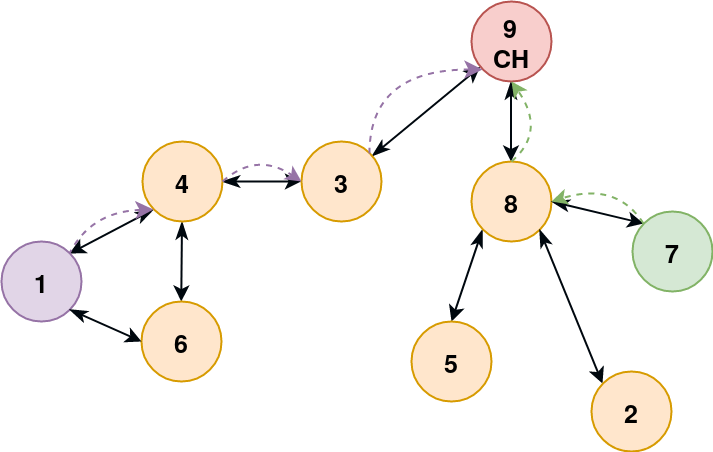
\includegraphics[width=\textwidth]{sendData.png}
%\caption{Figure show how a node sends its data to the leader through the nodes the path.}
%\label{fig:sendData}
%\end{figure}

\begin{figure}
\centering
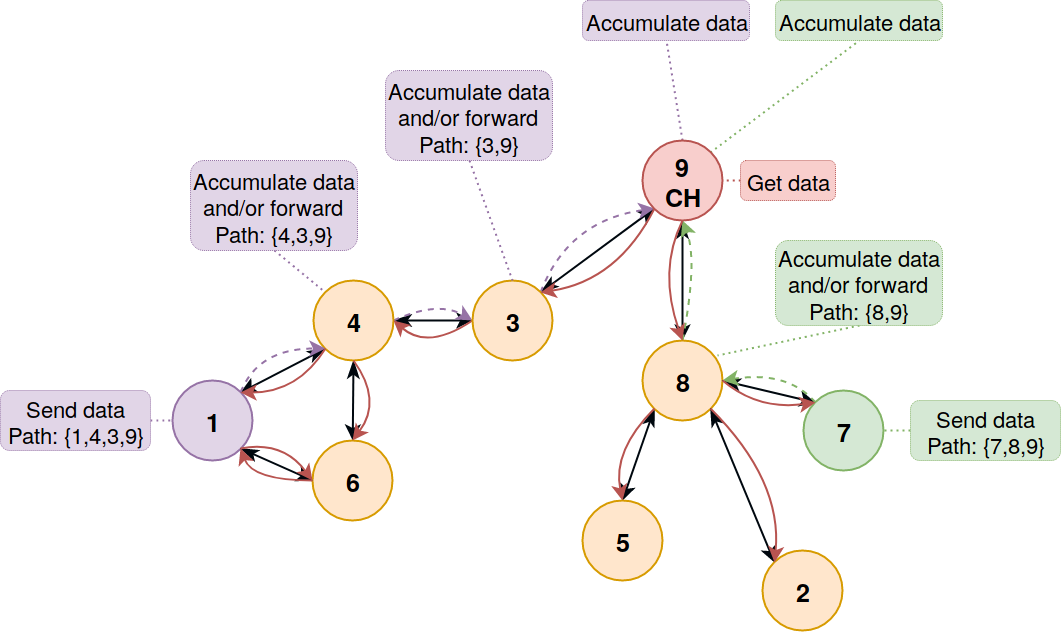
\includegraphics[width=\textwidth]{gatherSendData1.png}
\caption{Figure show how \gls{ch} gossips a GET-data request and how  nodes sends their data to the leader through the nodes in the path.}
\label{fig:gaterSendData}
\end{figure}

%\section{Base Station Access?}
%CH will keep data and send it to BS when it has access??
%CH changes so not


\chapter{Implementation} \label{chap:implementation}
\glsresetall
%Threads, data structures, language

This chapter will elaborate implementation of the system, general implementation requirements, issues and choices. 

The system is implemented in the open source programming language GO 1.9.3\footnote{\url{https://golang.org/}}. Each node is launched as an unique process and they communicate with each other by Golangs HTTP Server which listens on the \gls{tcp} network. The reason for using Golang is because it's developed for making concurrent mechanisms easy and to utilize multicore and networked machines, and it offers multiple different libraries. When nodes communicate with each other, they send packets structured as JSON \footnote{\url{https://www.json.org/}}.

Each node in the network has a limited battery lifetime and during execution the node's battery will be drained causing the node to eventually die. A \glspl{ch} battery lifetime will be drained faster to simulate that a \gls{ch} have potentially more tasks than a regular node.

It is not suitable to have nodes deployed in the Arctic Tundra at such an early development. This implementation simulates a real-life environment where nodes can communicate with each other through the \gls{tcp} network. Each node is assigned \textit{x,y} coordinates within a network grid size and a broadcast width, as shown in \ref{fig:broadcastNeighbour2}. The purple nodes are new nodes in the network and the purple arrows show connection between the new node and reachable nodes.


\begin{figure}
\centering
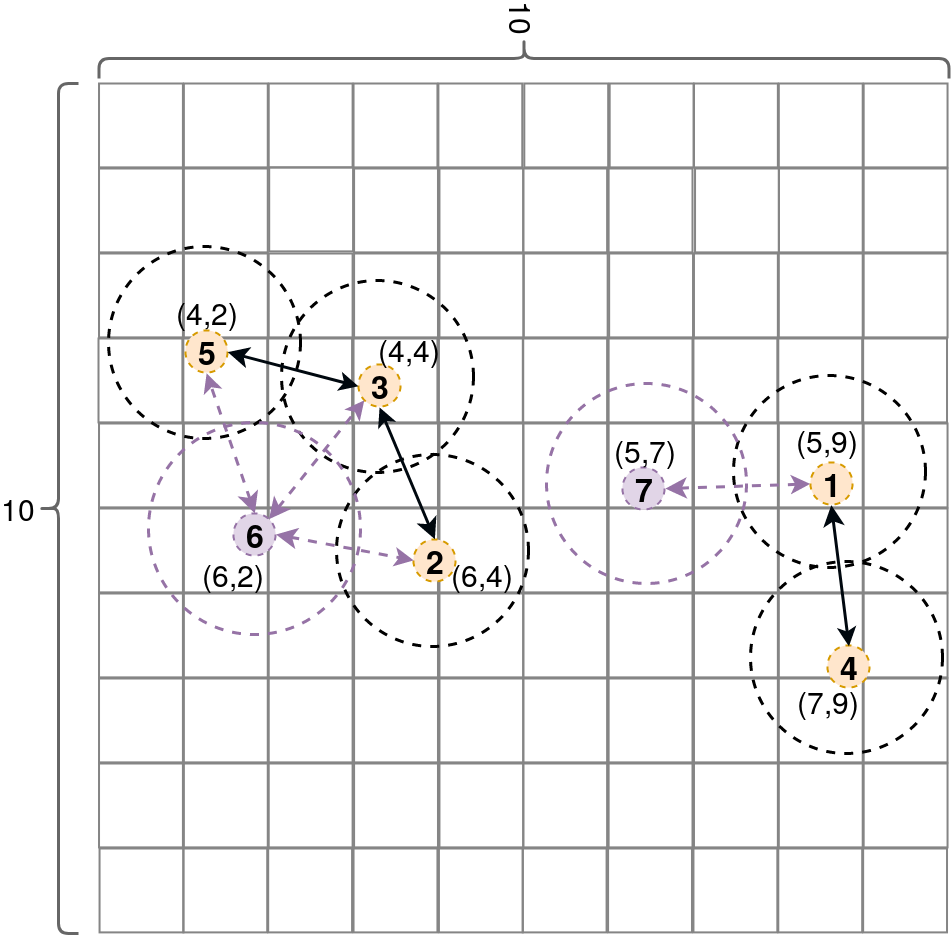
\includegraphics[scale=0.26]{contactNewNeighbour_3.png}
\caption{Figure show how the network grid size in scale 10 x 10 and nodes broadcast width.}
\label{fig:broadcastNeighbour2}
\end{figure}



\section{Distance To Other Nodes In The Network}
A new node will contact the lookup service to discover other nodes in the network by sending a POST-request containing meta-data about itself such as address and position (\textit{x,y} coordinates).

The distance formula \ref{eq:distance}, also called Euclidean distance \cite{euclidean}, is used to calculate the range between two points in a two-dimensional coordinate map and is used to see if a node is within a simulated radio range or not, as seen in Figure \ref{fig:broadcast_range}. The two points to be calculated is the position of the node itself together with the positions of all the running nodes in the network.

\begin{equation} \label{eq:distance}
d = \sqrt{(X_{2} - X_{1})^{2}+(Y_{2} - Y_{1})^{2}}
\end{equation}

%node attempt to connect..
\newpage

Figure \ref{fig:broadcast_simulation} shows how a node contacts the lookup service. The lookup service computes the node's position. Nodes within the simulated radio range is returned to the node. Finally, the node will try to connect to the these nodes.

\begin{figure} %[!b]
\centering
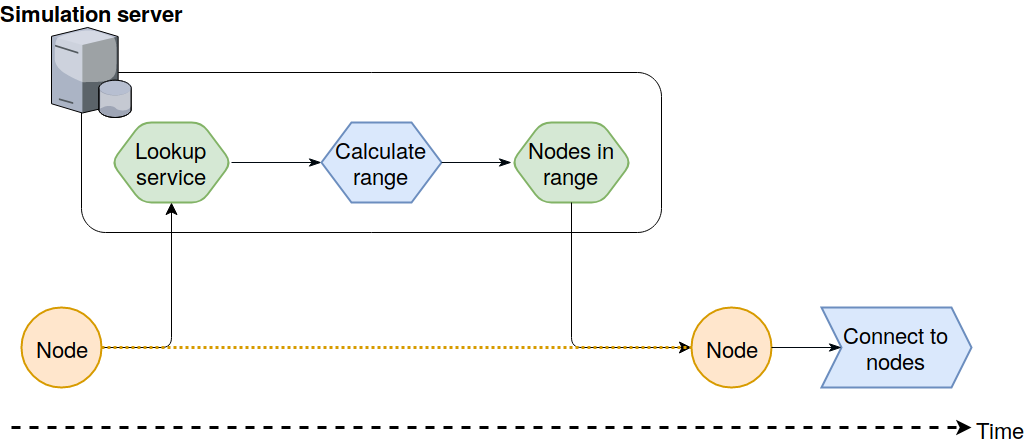
\includegraphics[width=\textwidth]{broadcast_simulation_kopi.png}
\caption{Broadcast simulation}
\label{fig:broadcast_simulation}
\end{figure}

\section{Connect To Neighbours}
A node will only be able to connect to another node in the network if the node accept the request to be neighbours. Presently, every node will be able to connect with their neighbours, as long as the node isn't unavailable by means of sleeping or if it's dead. There is no restriction in number of neighbours a node can have or that a node receiving a request from a new neighbour must forward the request to the \gls{ch} and let the \gls{ch} decide whether the new node can connect to the neighbour or not. Improvements to this approach is discussed in Section \ref{disc:conn_neighbours}. Figure \ref{fig:newNodeChart2} shows the flowchart of when a new node is created and when it will contact reachable neighbours and to start \gls{ch} election.


\begin{figure}
\centering
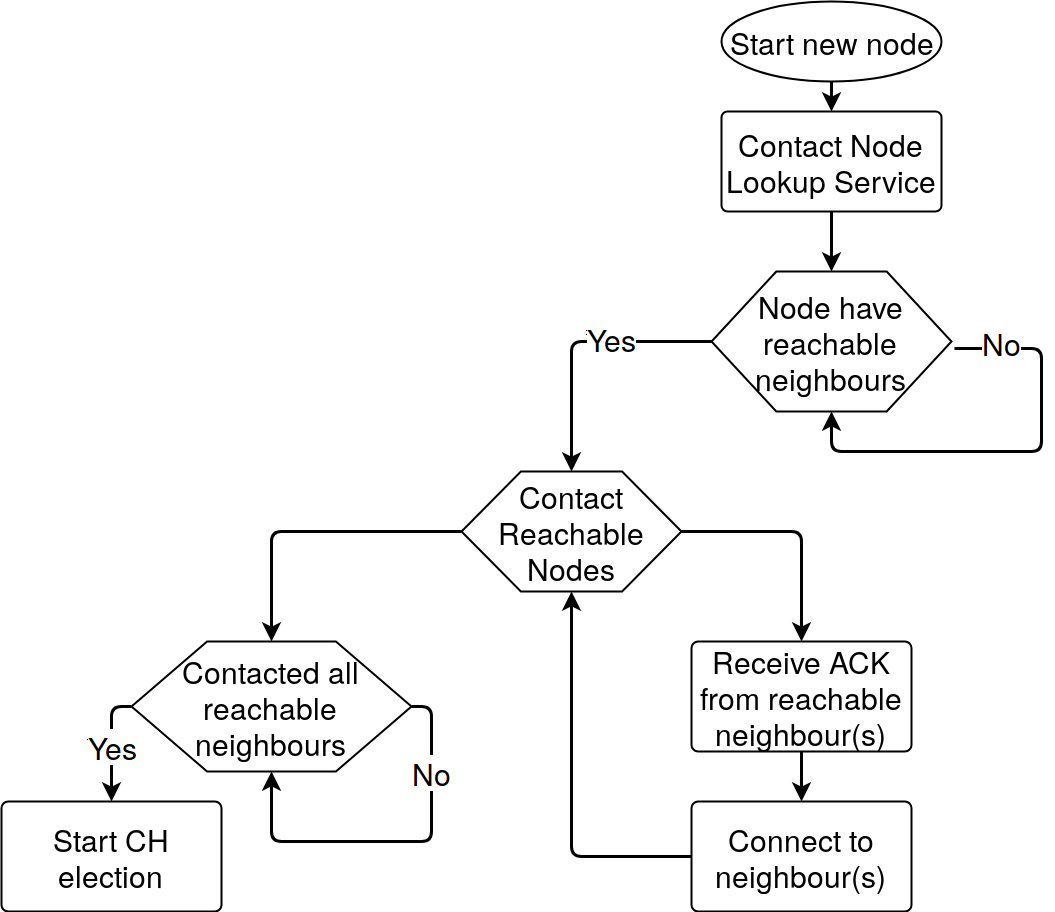
\includegraphics[scale=0.28]{newNodeChart2.png}
\caption{Figure show flowchart of when a new node is created and eventually starts a \gls{ch} election.}
\label{fig:newNodeChart2}
\end{figure}



\section{Cluster Head Election} \label{imp:ch_election}
%Leader election takes time to stabilize because of gossiping..
%Bully algorithm.. traditonially algorithm: nodes ON, we assume nodes OFF/our nodes most likely OFF.. 
%Gossip-based peer sampling - acm - mark jelasity \cite{gbsampling}


A \gls{ch} election is proposed either when a new node joins the network or by a \gls{ch}. 
The \gls{ch} election algorithm is based on the Bully algorithm \cite{bully} where typically the node with the highest ID number is selected to be the \gls{ch}. Our approach do not use the node with highest ID number, but elect the node with highest score by choosing a random value between $\emptyset$ and 1 to be a \gls{ch}. Each node makes its own decision about whether to become a \gls{ch} or not depending on the received score from neighbour nodes.
Our approach have several improvements discussed further in Section \ref{ssec:ch_election}. 

To avoid flooding the network, each \gls{ch} election round have an ID. If a node receiving an election have received a request with similar ID and the \gls{ch} haven't changed, the request will not be forwarded to other nodes considering that the node have forwarded the same request previous.

\subsection{Cluster Head Calculation}
To make the system more realistic in terms of battery lifetime and the capability to become a \gls{ch}, each node will receive a \gls{ch} computation request before an election if the \gls{ch} election is started by a \gls{ch}. This approach assumes that all nodes are possible candidates to become \gls{ch}s. This is to simulate that the nodes characteristics may change during execution and that a node that was highly capable to be a \gls{ch} before may not be efficient in the next \gls{ch} election.


\section{Minimize Path To Cluster Head}
Since \gls{ch} elections are gossiped from all nodes, each node can receive multiple gossips per \gls{ch} election and some paths will be longer than others. In order to minimize the path to the \gls{ch}, a node will when receive an election, compare its existing path to the one received \cite{dijkstra} and choose the shortest path to be its path to the leader.

%Finiding a path to the \gls{ch} is based on Dijkstra algorithm to find the shortest path between two nodes \cite{dijkstra}.

%network traffic, nodes energy/battery, 

%\cite{multiradio}: The goal of the metric is to choose a high-throughput path between a source and a destination.


\section{Data Accumulation}
%fabricated data 

%mediated = try to bring to an agreement

\subsection{Node Data Accumulation}
Since all nodes run concurrently and independently, each node can receive multiple requests from different neighbouring nodes. When a \gls{ch} creates a request for gathering data will the request contain an ID used for identification. Since the request is gossiped to all nodes in the cluster, a node will most likely receive the same message multiple times, but only need to forward its data once. If a node have not received a request with a specific ID, it will gossip the message to its neighbours and then send its data to the next neighbour in the path to \gls{ch}. Otherwise, the node will just ignore the request.

When a node needs to send data, it will create a request containing the received request-ID from the \gls{ch}, the data to be sent together with a fingerprint and a path to the \gls{ch}. The path to the \gls{ch} is a list containing the addresses for the nodes between the sender and the \gls{ch}.

%JM: hva skjer hvis en node feiler eller blir borte? restart av melding?

The data is a fabricated byte array with a fingerprint that is the hashed value of the data. The fingerprint will make it easier to identify the numerous data on each node. The data will also have a boolean tag which is used to check whether the data has been accumulated or not. 
%JM: endrer det hash?


\subsection{CH Data Accumulation}
When a \gls{ch} starts a gathering of data, the node will chose a value between one and six which indicates how many times it should gather data before it eventual sends out a new \gls{ch} election. We chose to implement the \gls{ch}s to accumulate data between one and six times because finding the exact number of how many times a \gls{ch} should accumulate data wasn't our focus.

%We chose to focus on the network and how nodes performed during \gls{ch} elections and data accumulations instead of finding the exact number for how many times a \gls{ch} should accumulate data.


As mentioned previously, each node can receive multiple requests from different neighbour nodes.
This especially occur in the \gls{ch} when collecting data from the nodes in the cluster. The collected data is stored in a map and maps in Go are not safe for concurrent use. If a map is read from and written to from concurrent goroutines, the access must be synchronized. One of the most common ways to protect maps is by using mutexes, illustrated in Listing \ref{test}.

%\newpage

\begin{lstlisting} [frame=single,caption={Small Go program showing how mutexes are used when updating a map by CH.},language=C, label={test}]

/*SensorData is data from "sensors" on the OU */
type SensorData struct {
	ID          uint32
	Fingerprint uint32
	Data        []byte
}

/* DBStation is a strucure that contains 
   a map that store data at CH */
var DBStation struct {
	sync.Mutex
	BSdatamap map[uint32][]byte
}

func sendDataToLeaderHandler() {
	var rd SensorData
	
	DBStation.Lock()
	defer DBStation.Unlock()
	
	(...)
	
	err := json.Unmarshal(body, &rd); 
	if err != nil {
		panic(err)
	}
	
	(...)
	
	/*Update map in key FingerPrint
	  with received data */
	DBStation.BSdatamap[rd.Fingerprint] = rd.Data
}
\end{lstlisting}


\newpage

\section{Concurrent CH Election And Data Accumulation} \label{sec:conc_events}
To avoid having a \gls{ch} election occur concurrently with a data accumulation, the following functionalities are scheduled to execute.
Firstly, the \gls{ch} election will execute until the election result is consistent between all nodes.Second, the \gls{ch} broadcast a request for gathering data and nodes will accumulate and send data to the \gls{ch}. Third, after gathering data according to the accumulation interval, the \gls{ch} starts a new \gls{ch} election. 

\textbf{Hvilke issues??}

If a \gls{ch} election and a data gathering happens concurrently, there may be issues when the node is supposed to send its data because the \gls{ch} may have changed and the path to the \gls{ch} may be incorrect. 


Our approach to a solution to this interference is to have the two functionalies divided into different phases similar to \gls{leach} \cite{leach}, described in Chapter \ref{chap:related_work}. Timers are implemented to stall the next phase by making the system sleep until the timer is ended. This issue and improvements are discussed further in Section \ref{disc:simult_el_acc}.


%\textit{JM: kan du utvide dette til a virke med failed nodes?}


%\section{Base Station Access}



\chapter{Evaluation}
\glsresetall
This chapter describes the experimental setup and metrics used to evaluate the implemented system.

\section{Experimental Setup}
All experiments were done on a Lenovo ThinkCenter with the following specifications:

\begin{itemize} 
\item Intel® CoreTM i5-6400T CPU @ 2.20GHz × 4
\item Intel® HD Graphics 530 (Skylake GT2)
\item 15,6 GiB memory and 503 GB disk \textbf{eller GIB??}
\item Ubuntu 17.04 64-bit with gcc V6.3.0 compiler and GO 1.9.3
\end{itemize}


The environment for \textbf{evaluating/testing} our system is built with gopsutil, a psutil for Golang \cite{golangPsutil}. We use gopsutil to measure CPU, memory, network and process connections. Each experiment is described further in Section \ref{eva:exp_des}.

\section{Experimental Design} \label{eva:exp_des}
\textbf{
How did we do the experiments?
For hvert eksperiment bør du prøve a fa fram: 
\begin{itemize}
\item hva ønsker du a finne ut?
\item hvordan måler du + hva måler du? 
\item hva gjør den delen av systemet som du måler? (leser fra disk, regner, sammenligner, koordinerer med andre osv)
\item Hva er metrikken (eks: operasjoner per sekund, minutter per oppgave osv)
\item Det gjør det lettere for leseren a henge med.
\end{itemize}
}

All experiments were conducted on a computer, where a process is simulating an \gls{ou}. In order to determine memory, CPU and network usage, several experiment scenarios were designed and performed.

%execute around 15 minutes
\textbf{Forklar (hva menes + why)}

The experiments are ran with a 500 millisecond's measurement interval because  ... 

The system execute minimum 10 minutes. The experiments are done executing 100 nodes with a broadcast range at 50, as shown in Table \ref{tab:simTable}. During execution, the nodes in the system will communicate between each other, gossip \gls{ch} election and store and accumulate data both between themselves and at \gls{ch}s.

\begin{table} [ht]
\centering
\begin{tabular}{|l|l|}
\hline
\textbf{Parameter}       & \textbf{Value} \\ \hline
Number of nodes          & 100            \\ \hline
Network grid size        & 500 x 500      \\ \hline
Node broadcast width     & 50             \\ \hline
\end{tabular}
\caption{Parameters of simulation}
\label{tab:simTable}
\end{table}

\textbf{Forklar bedre - trenger repeterbare exp..}

Each node execute their own experiment when launched. Each time interval (500 millisecond) also \textbf{contains} an average value which is displayed in the graphs. \textbf{Fjerne?? Since each experiment is launched  independently, the clusters in the network may appear different in each experiment causing nodes to have more or less neighbour nodes and a longer or shorter path to the \gls{ch} than in another experiment.}


A \gls{ch} will chose a value between one and six which indicates how many times it should gather data. The experiments are ran on 4 different accumulation intervals as listed below:

\begin{itemize}
\item \gls{ch} accumulate data two times
\item \gls{ch} accumulate data four times
\item \gls{ch} accumulate data six times
\item \gls{ch} accumulate data a random time between one and six times
\end{itemize}

%Notes to myself: Each node execute their own experiments when launched.. graphs shows average.. too much with 100 lines in a graph...
%For each time interval (500 millisecond), the average value was calculated to limit the 
%Test were/was conducted X times for each time period in order to obtain the average values...


\subsection{Memory Measurements} \label{eva:mem_measure}
%discover/observe/see
We measure the memory usage to examine how much memory is consumed when executing our system. The memory usage measured, is the total percentage of RAM used by the program, and not for individual processes. The memory usage is essential to examine because it ...
% to be relatively low to be able to make the device function as normal in a real-life environment/scenario.

\begin{itemize}
\item \textbf{Psutil - VirtualMemoryStat - UsedPercent:} percentage of RAM used by programs.
\end{itemize}



\subsection{CPU Measurements} \label{eva:cpu_measure}
We measure the total CPU usage for the computers four cores combined to document how much computational power is needed to execute the program. This means that the CPU usage is similar for all nodes/processes in the experiment.
This as well, is important to keep at a minimum due to execution on devices in real-life environment to avoid draining the battery.


\begin{itemize}
\item \textbf{Psutil - Percent:} calculates the percentage of CPU used either per CPU or combined.
\end{itemize}


\subsection{Network Usage} \label{eva:net_measure}
%psutil - ConnectionPid - Return a list of network connections opened by a process. 
%\subsection{Process Connections Measurements}
%psutil - Process 

We measure the number of process connection since the system relies on network usage and communication between nodes and it is important to keep it to a minimum. The number of communication channels are represented by open sockets that a node have open at any given point. These open sockets may be because of discovery of other nodes, \gls{ch} election, forwarding- and data accumulation.

\begin{itemize}
\item \textbf{Psutil - ConnectionsPid:} Return a list of network connections opened by a process.
\end{itemize}


%\subsection{Network Lifetime?}

\subsection{Number Of Sends To Neighbours} \label{eva:num_sends}
We measure number of sends to neighbours to \textbf{measure/calculate} the number of sends between nodes in the system during execution. This experiment is in connection with the network usage and communication, described in Section \ref{eva:net_measure}. The number of sends are counted every time the node sends a request to a neighbour, like discovering other nodes, connecting to other nodes, \gls{ch} election or sending and accumulating data to \gls{ch}.


\subsection{Number Of Sends To Cluster Heads} \label{eva:num_sends_ch}
We measure the number of sends to a \gls{ch} during execution. The number of sends are only counted when there is a accumulation request to send data to a \gls{ch}.

As described in Section \ref{eva:net_measure}, are communication between nodes and network usage important to keep to a minimum. Besides measuring number of sends to neighbours, we measured number of sends to a \gls{ch} during execution. The number of sends are only counted when there is a accumulation request to send data to a \gls{ch}.


\subsection{Cluster Head Count} \label{eva:ch_count}
We measure how many times nodes have been \gls{ch}s at each time interval to examine if how many \gls{ch} there is at each time interval. The \gls{ch} is only counted when it's done gathering all the data.


\subsection{Cluster Head Receives Packages} \label{eva:ch_recv}
We measure how many times a \gls{ch} receives data from other nodes in the network. This is measured only at each \gls{ch}. We want to measure this to examine the difference between the number of sends to a \gls{ch} and how many times a \gls{ch} have received a packet.

\newpage

\section{Results}
%There is reason to think that (this implementation)...
%A thing to mention, is that ...

%What does the results say?
In this section we will present and discuss the results of the experiments described in the sections above.

\subsection{Memory Usage}
%random acc gives the least memory usage.. - mem 6 acc gives highest acc, not suprising becayse it does most wirtes to memory when accumulating data.. Otherwise, pretty similar memory usage.. no spikes or 

The purpose of this experiment was to examine how much memory the system consumes when executing the program. The result is presented in Figure \ref{fig:memChart}. We can see that the system have between 60\% and 76\% memory usage and the graphs shows that each experiment us approximately the same amount of memory. However, there is one graph that stands out, which is the graph showing the memory after a random number of accumulations.
There is reason to think that this implementation uses less memory than the others because the accumulation intervals are more distributed during execution in contrast to the other accumulation intervals where all \gls{ch}s accumulated data appropriately at the same time interval. As for the experiment for the implementation with six accumulations, the memory percentage is the overall highest of all experiments. We can assume that this is because of the most amount of accumulation causing the \gls{ch} to use more memory.


\begin{figure} [ht]
\centering
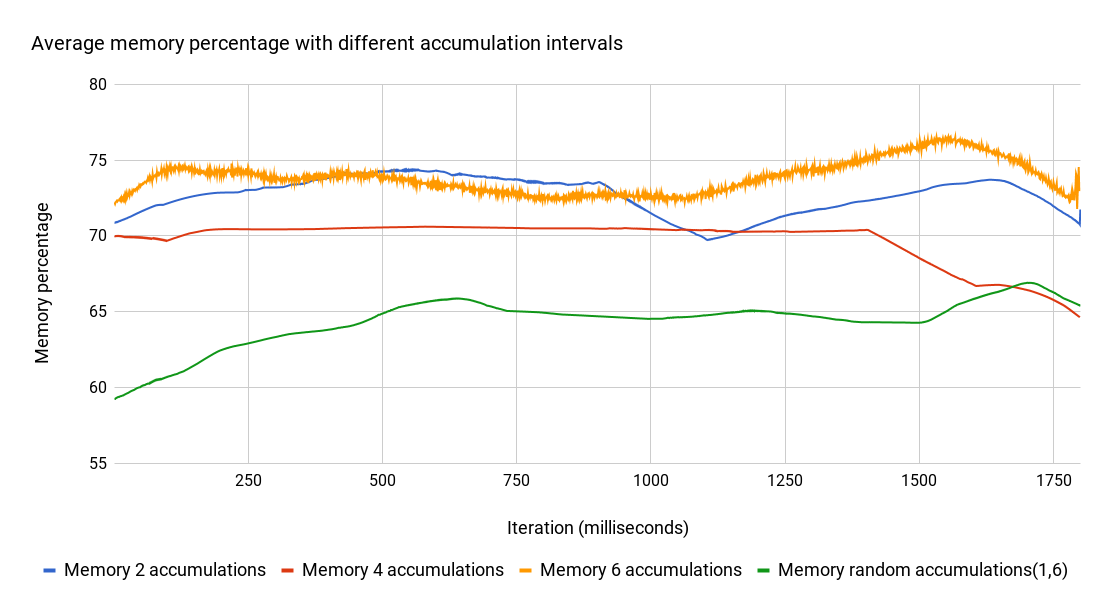
\includegraphics[width=\textwidth]{memChart2.png}
\caption{Figure shows average memory percentage with different accumulation intervals (500 milliseconds).}
\label{fig:memChart}
\end{figure}


\subsection{CPU Usage}
We measured the CPU utilities to examine the CPU percentage of the system. As we can see from Figure \ref{fig:cpuChart}, the CPU percentage is between 40\% and 95\% during execution and each experiments uses approximately the same amount of CPU.
The CPU percentage is stable on around 75\% during the execution for each experiment. We believe that the reason there is no peaks during execution, is because of Golangs\footnote{\url{https://golang.org/}} ability to utilize multicore and networked machines. Another reason for the graphs being so stable can be because the nodes are waiting for a request to either accumulate data or elect a new \gls{ch}. Most of the execution time, the nodes are waiting for requests.


%\textit{Note to self: Starting nodes, elect leaders, gather data after some time.., eventually elect new leader, and gather data again..may be that clusters are so "small" that they do not make any crazy things about CPU. More nodes connected - more CPU usage?? also golang that utilize multicore and networked machines..? nodes running and waiting for requests.. should probably peak when ch electing or data accumulation.. but maybe golang is the shit..}


\begin{figure} [ht]
\centering
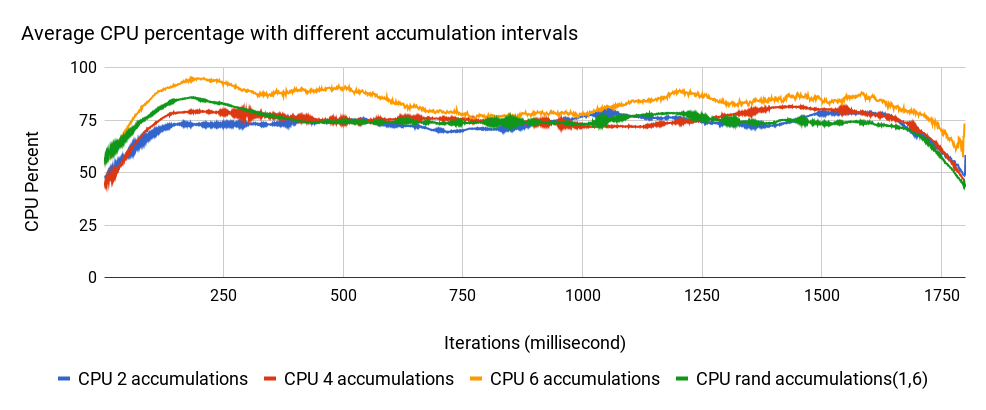
\includegraphics[width=\textwidth]{cpuChart.png}
\caption{Figure shows average CPU percentage with different accumulation intervals (500 milliseconds).}
\label{fig:cpuChart}
\end{figure}


\newpage

\subsection{Network Usage}
The purpose of this experiment was to measure the network usage and communication between nodes since it's important to keep this to a minimum since it's aimed to execute on small, low-power \gls{ou}s. The result is presented in Figure \ref{fig:netconnChart} and show a wave like pattern. The number of connections in the system range from 1 connection to 11 connections on average per node for 100 node in the system.
There is reason to believe that these high wave like patterns showing a high amount on connections is because of three reasons:

\begin{itemize}
\item Firstly, nodes are created and communicate with reachable nodes to connect to and eventually starts a \gls{ch} election resulting in a high amount of connections.
\item Second, when a \gls{ch} broadcasts a message that a data accumulation should be started, the message is broadcast to every node in the cluster resulting in many open connections.
\item At last, after accumulating data from other nodes in the cluster, the \gls{ch} gossip a new \gls{ch} election calculation and then gossip a new \gls{ch} election.
\end{itemize}

There is also reason to think that these wave like patterns occurs at different time intervals is because of the different implementations accumulate data and elect \gls{ch} at different time intervals.

%around 6 connections are average..

\begin{figure} [ht]
\centering
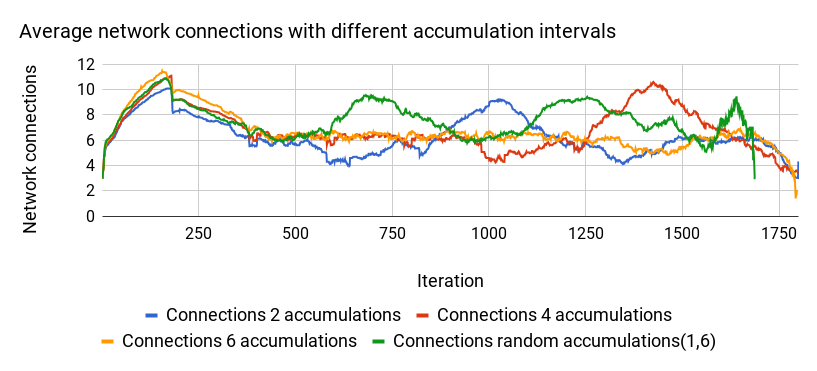
\includegraphics[width=\textwidth]{netconnChart.png}
\caption{Figure shows average network connections with different accumulation intervals (500 milliseconds).}
\label{fig:netconnChart}
\end{figure}


\newpage 

%\subsection{Network Lifetime?}
\subsection{Number Of Sends To Neighbours}
Since it's important to keep communication and network usage to a minimum, we measure the number of sends from nodes to neighbours. 
As we can see from Figure \ref{fig:sendsChart}, will number of sends from one node to another increase during execution. The average number of sends from nodes range between 1 send up til around 95 sends. This is an expected result since each time a node communicate with another node, it's counted and therefore will increase during execution.
As mentioned in Section \ref{eva:exp_des}, the different experiments are ran independently causing the nodes in the network to create clusters with different number of cluster members. There is one graph-line that stands out compared to the three others. There is reason to believe that the result of accumulating data four times have a higher average of sends between nodes because the nodes in clusters in this experiment had more neighbour nodes and possibly a longer path to the \gls{ch} when accumulating data.

\begin{figure} [ht]
\centering
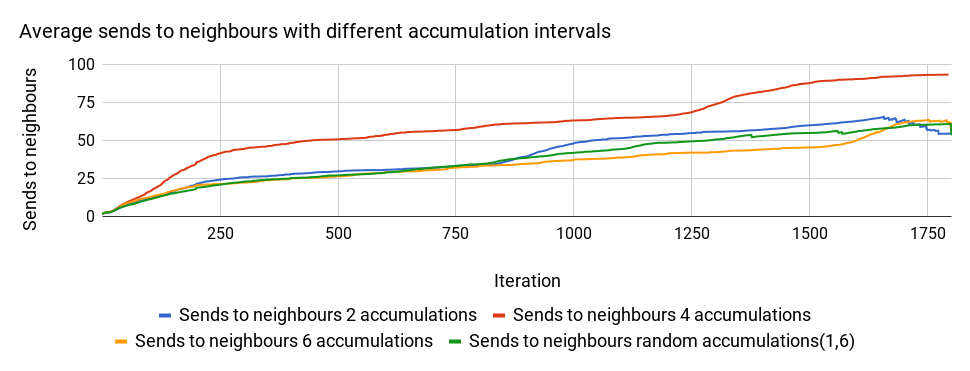
\includegraphics[width=\textwidth]{sendsChart.png}
\caption{Figure shows average number of sends from nodes to neighbour nodes with different accumulation intervals (500 milliseconds).}
\label{fig:sendsChart}
\end{figure}


\newpage

\subsection{Number Of Sends To Cluster Heads}
Number of sends to \gls{ch}s is also connected to the experiment  with communication and network usage. The result is presented in Figure \ref{fig:sendschChart} where we can see that the number of sends to \gls{ch}s increase during execution. This is also an expected result in thought of the \gls{ch} are gathering more and more data. The average number of sends to \gls{ch} range between $\emptyset$ sends up til around 35 sends.


%her også avhenger hvert experiment på hvordan nodene har laget cluster.. ch kan ha hatt fler eller ferre naboer og flere eller ferre noder i clusteret..

\begin{figure} [ht]
\centering
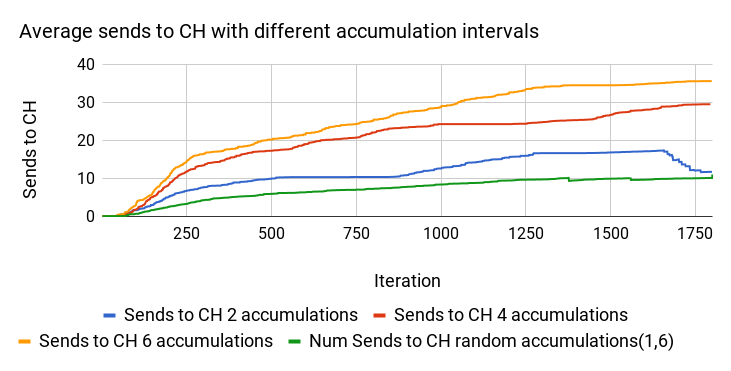
\includegraphics[width=\textwidth]{sendschChart.png}
\caption{Figure shows average number of sends to \gls{ch}s with different accumulation intervals (500 milliseconds).}
\label{fig:sendschChart}
\end{figure}


\newpage

\subsection{Cluster Head Count}
%Flat/stabilt nar node venter pa a same data igjen.. da venter ogsa de andre nodene.. vil bare øke etter X accumualtions.. 

The result is presented in Figure \ref{fig:chCountChart}. The graphs are as expected flat during parts of the execution because the \gls{ch}-count is only counted when the \gls{ch} is done gathering data.
There is reason to think that the all graphs, except the graph of \gls{ch}-count after a random number of accumulations, have flat graphs during execution because all the \gls{ch}-counts happens approximately at the same time interval and don't change until the next \gls{ch} election.
Counting the number of \gls{ch} after a random number of accumulations, show a more increasing graph during execution because of the accumulations happens at different time interval causing the \gls{ch} election to be more spread during execution.

\begin{figure} [ht]
\centering
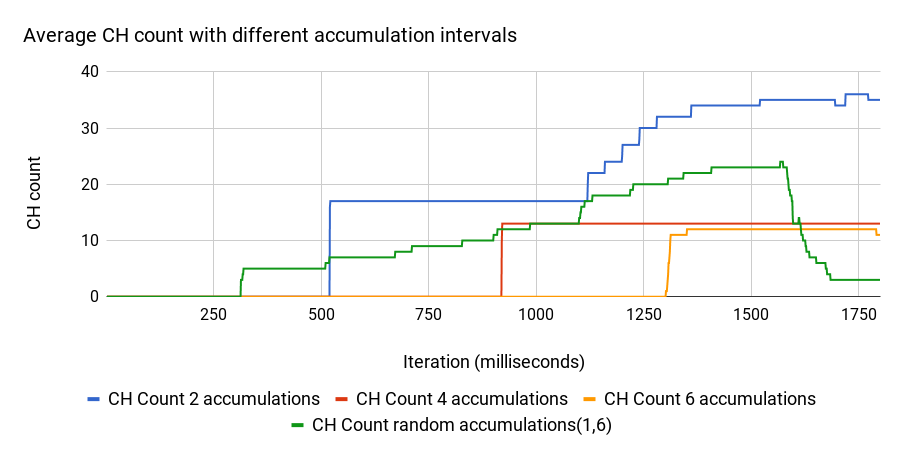
\includegraphics[width=\textwidth]{chCountChart.png}
\caption{Figure shows average number of \gls{ch} with different accumulation intervals (500 milliseconds).}
\label{fig:chCountChart}
\end{figure}


\newpage

\subsection{Cluster Head Receives Packages}

As we can see from Figure \ref{fig:recPktChart}, are the number of packets \gls{ch}s receives relatively similar during each experiment. This result as well, is expected because the \gls{ch}s will receive more data each time they ask for it.

\begin{figure} [ht]
\centering
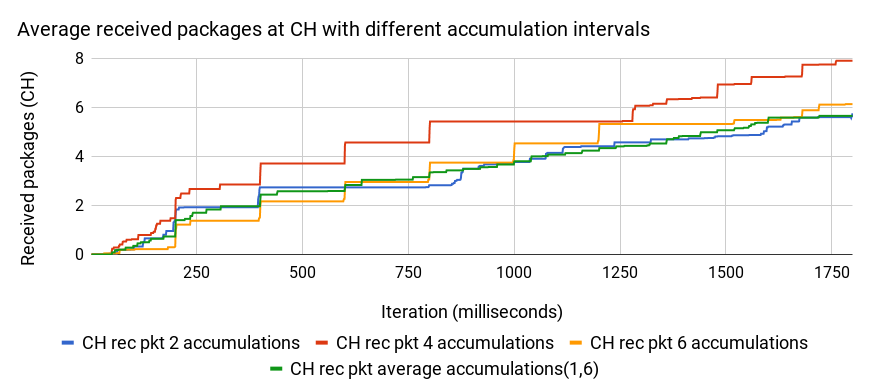
\includegraphics[width=\textwidth]{recPktChart.png}
\caption{Figure shows average number of \gls{ch} with different accumulation intervals (500 milliseconds).}
\label{fig:recPktChart}
\end{figure}



Figure \ref{fig:sentvsrecvChart} show the number of sends from nodes to neighbours, sends from nodes to \gls{ch}s and number of times \gls{ch}s have received data. As we can see, are the number of received packets less than sends to \glspl{ch}. It is therefore reason to think that the nodes accumulate data to reduce the number of packets a \gls{ch} receives.

%mye dat blir accumulert - resulterer i lavere ant recv enn sends.. det er jo bra!

\begin{figure} [ht]
\centering
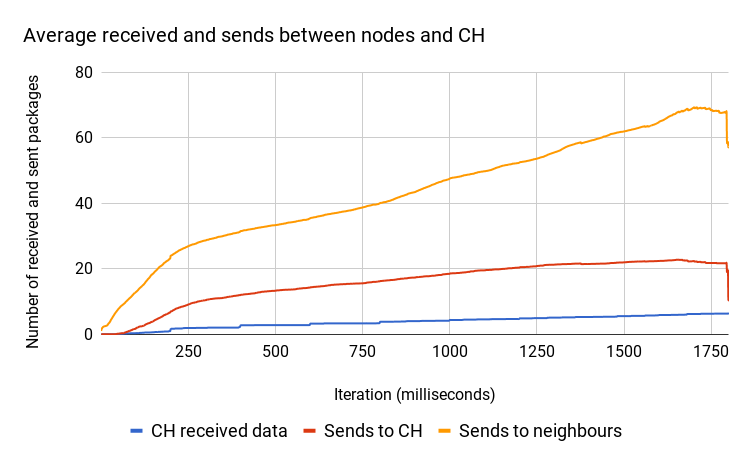
\includegraphics[width=\textwidth]{sentVsRecvChart.png}
\caption{Figure shows average number of \gls{ch} with different accumulation intervals (500 milliseconds).}
\label{fig:sentvsrecvChart}
\end{figure}




\chapter{Discussion}
\glsresetall
%There is reason to think that (this implementation)...
%A thing to mention, is that ...
%One can assume

%Idea, arch, design, results, other solutions, "arch has scale issue"..
This chapter discusses our approach, experiences, how we solved the problem and why we chose the solution we ended up with.

\section{Availability Of Nodes In The System} \label{disc:node_conn}
%ambigious - tvetydig, open to more than one intepretation
%krav

\subsection{Connect To Neighbours} \label{disc:conn_neighbours}
%When a node wants to join the cluster, should it ask the CH or should it join eitherway.. What if CH is sleeping (or busy) so that it's not reachable, or that nodes in the path to CH are sleeping (then how to contact CH?)..

% CH elect if node can join cluster or not...

In the current approach a node can connect to nearby nodes and be a part of a cluster without any restrictions. In our first approach when a node received a request from a new node, would forward the request to the \gls{ch}. The \gls{ch} then determine if the new node is allowed connect to the cluster or not. However, making a \gls{ch} take this decision could be problematic because the \gls{ch} needs to know information about the whole network or at least its own cluster, and also need some requirements for when a node can join and not. Some requirements that a \gls{ch} can consider are:

\begin{itemize}
\item Number of nodes per cluster
\item Number of neighbours a node can have
\item Distance from new node to \gls{ch}
\item Node characteristics (bandwidth, energy level, memory etc.)
\end{itemize}

Another interference with having a \gls{ch} take the decision is that the \gls{ch} may be unavailable because it's sleeping or if it's unreachable because nodes in the path to the \gls{ch} are sleeping or unavailable due to e.g. saving battery. 

%Ping othern nodes regulary to check if neighbours are alive or not, or ping right befre a sending of data to ch.. what if a node in the path to leader is dead? what if there is no other way to the ch? what happens? 
\subsection{Ping Neighbours}
An improvement to check if neighbours are alive or not, is to ping neighbouring nodes frequently to check if they are alive or not/\textbf{there is any response}. However, pinging other nodes frequently will eventually flood the network. An improved solution is to only ping neighbours if there is a need for communication between nodes. For example to ping neighbours before forwarding a message to the \gls{ch}. This ping-request will most likely contain a wake-up call to the next node in the path to the \gls{ch} so nodes are awake when receiving a forwarding request to the \gls{ch}.

%how to know if node is dead or just sleeping


\subsection{Node Waking Up After Sleeping/Being Unavailable}
%What if nodes are regulary off/sleep, how to know which one is ch? ask neighbour, and each election have an id/timestamp to check if this is the last election.. Could be that there have been multiple ch electins while node has been asleep so the neighbour node have not the right ch according to other nodes..
%global clock so each node knows when to awake to send data to ch or leader election, etc..?

%Right now: no timestamp or regulation.. If node down, it will send its data to the node he think is the leader, but that is not all bad because data will be send do the leader/gather eventually anyways.. Maybe next round or something.. but improvement: have timestamps or global clock - vector clock..

%Should remember old leader.. or old leader should know that it has been a leader and have data to be sendt to the bs..

%multiple solutions: ask neighbours, hvis ulike svar, tell hvilket svar som det er flest av, ha timestamp pa election

At the current approach, there is no timestamp or schedule for when the \gls{ch} was elected. If a node was unavailable during the \gls{ch} election, it will most likely forward its data to the old \gls{ch}. However, this isn't necessary a drawback since the node receiving this data will forward the accumulated data in the next gathering phase.
To improve this approach and avoid inconsistency of the \gls{ch}, we could implement a solution to ask the nodes neighbours who the \gls{ch} is. Each \gls{ch} election should have a timestamp to compare in case the node receives multiple different answers. Then the node could compare the different timestamps and choose the timestamp that is the biggest or the closets to its own clock, depending on the implementation. 

%Another approach is to have an consensus protocol for agreeing on a leader. This approach, together with other possible solutions for electing a new \gls{ch}, is discussed further in Section \ref{disc:ch_election}.


\section{Cluster Head Election} \label{disc:ch_election}
Being a \gls{ch} is more energy intensive than being a regular cluster node because it may transfers data over longer distances and performs more tasks. If the \gls{ch} is chosen a prior, meaning the \gls{ch} is chosen before the nodes have knowledge of each other and created clusters, e.g. by a \gls{bs} without any knowledge about the network, then the node would quickly use up its limited energy. Once a \gls{ch} runs out of battery, it is no longer operational and all nodes belonging to the cluster will lose their communication ability. To avoid this problem, our approach will not chose \gls{ch}s a priori, but instead have a \gls{ch} election algorithm to possibly rotate the \gls{ch}.


%\subsection{Consensus Protocol For Elections?}


\subsection{Cluster Head Calculation} \label{ssec:ch_election}
Presently, the \gls{ch} election is based on which node has the highest score between $\emptyset$ and 1. This intentionally simplified does not take in account many other realistic aspects which would improve the \gls{ch} election. To improve this approach and make it more realistic in terms of saving battery lifetime and a real-life scenario for deploying sensors in the Arctic tundra, we could have used several sub-factors listed below:

\begin{itemize}
\item Number of nodes between a node and \gls{ch}
\item Number of neighbours for the node
\item Access to \gls{bs}
\item Power left on node
\item Bandwidth - WiFi, LoRaWan\footnote{\url{https://lora-alliance.org/about-lorawan}}, Ethernet
\item Prior history
\item Network traffic on node
\end{itemize}

%Bully algorithm.. traditonially algorithm: nodes ON, we assume nodes OFF/our nodes most likely OFF.. 

%Er det bare en function-endring eller er det også spørsmål om du har nødvendig info?


%\subsection{Eventual Cluster Head Election Consistency?}



\subsection{Gossip Information Between Nodes}
%rapidly, maybe not always.. kommer an på
The main advantages of gossiping is its ability to scale. Gossiping have no centralized component where information is coordinated and is therefore an excellent way to rapidly spread information among a large number of nodes using only local information. However, gossiping can not guarantee that all nodes will receive the information \cite{demers}.

To avoid flooding the network, each message sent between nodes have an ID so the node can check if it has received the same message before. If the node have received the message earlier, the node doesn't need to forward the message because it has forwarded the message in an earlier gossip, as described in Section \ref{imp:ch_election}.

\newpage

Another approach to avoid flooding the network and reduce nodes energy level is to limit the number of hops when gossiping to other nodes. To avoid this flooding can each packet have a hop count and every time a packet hops, its hop count increment. When a packet's hop counts equals a hop limit, the packet will be discarded. Flooding the network with updates as the current approach does, ensures eventual consistency.
 
 
\subsection{When To Elect A New Cluster Head}
The present approach starts a new \gls{ch} election in two scenarios: either when a new node joins the cluster or when the \gls{ch} have accumulated data 'X' times. Other approaches such as \gls{leach} \cite{leach}, mentioned in Chapter \ref{chap:related_work}, have multiple phases during execution where one phase is to elect a new \gls{ch} which occurs periodic.

%every other = annenhver

The current approach is similar to \gls{leach} using different phases for electing a new \gls{ch} and accumulate data. We chose this solution because of concurrency issue when these two events happen at the same time, as mentioned in Section \ref{sec:conc_events}. This issue is also discussed further in Section \ref{disc:simult_el_acc}.

%Improvements??
%JM: en mulig sak hva skjer hvis CH fpr X mndinger samtidig som en eller fler andre vil sende? er dert ch som initere query bestandig eller kan andre bestemme seg for a sende?


\section{Remember Previous Cluster Head}
At the present approach, nodes do not know that they have been \glspl{ch} in an earlier election. The nodes should know if they have been elected to \glspl{ch} earlier because they have accumulated data from other nodes in the cluster. This data should be sent to a \gls{bs}. The \glspl{ch} can have access to a \gls{bs} during their whole lifetime or at some points during their lifetime. Access to \glspl{bs} are discussed further in Section \ref{disc:bs_acc}

To improve our current approach, each \gls{ch} should remember that they have been elected as \gls{ch} in an earlier election. Eventually, when the \gls{ch} have been in contact with a \gls{bs} that collects all the \glspl{ch} data, they can forget that they have been \glspl{ch} and also remove their data to increase memory capacity.


%remember CH status so data can be sent to BS/drone...


\section{Multiple Cluster Heads} \label{disc:multi_ch}
%multiple leaders load balance the network and nodes with work.. shorter path to leaders for some nodes
The current approach have only one \gls{ch} per cluster. If there are many nodes in one cluster, there can be a lot of work load for the \gls{ch}, and the path to the \gls{ch} can be long for some nodes.
An improvement to this is to introduce multiple leaders to load balance work and may also provide shorter path for some nodes. The question is then which \gls{ch} should a node choose to be its \gls{ch} if there are multiple. \gls{ch} elections will be based on several sub-factors described in Section \ref{ssec:ch_election}. If we assume that all nodes that are qualified to become \gls{ch}s are equivalent in terms of battery lifetime, network bandwidth and number of neighbours, the node should choose the \gls{ch} with the shortest path to avoid flooding the network with requests and to avoid draining the limited energy on more nodes than necessary. Having multiple \glspl{ch} that accumulates data would also support scalability and perofrmance issues in terms of balance work load between \glspl{ch}.


\section{Path To Cluster Head} \label{disc:ch_path}
One advantage with the present approach is that the \gls{ch} election chose the shortest path from a node to the \gls{ch} to avoid flooding the network with requests. The idea to use the shortest path \cite{dijkstra}, is presumably not beneficial to change in any approach. However, it may be that some nodes in a path to the \gls{ch} have a limited battery lifetime and therefore should not be in a path to the \gls{ch}. This is a corner case which will be difficult to give a right answer to since the paths and nodes can occur in many different scenarios.

%avoid flooding
%minimize path to leader


\subsection{Multi-hop or single-hop routing} \label{disc:hopping}
%https://en.wikipedia.org/wiki/Multi-hop_routing

\gls{wsn} consists of hundreds or thousands of low-cost micro-sensor nodes and their main task is to collect information of the interested area and broadcast the information to a \gls{bs}. An easy approach to achieve this task is to make each sensor node transmit their data directly to the \gls{bs}, as Figure \ref{fig:hopping} shows. However, the problem is that the \gls{bs} may be places far away from the sensor node so a direct transmission would not be possible. Another problem can be that the routing path from a sensor node to the \gls{bs} is long and the node will require more power consumption than available.

In some cases can multi-hop routing be more energy efficient than single-hop routing\cite{hopping2}. Our approach is currently using multi-hop routing to deliver accumulated data to the \gls{ch}. To use single-hop routing in our approach would not be efficient in terms of energy consumption or sensor nodes radio range. In a real-life scenario where nodes are deployed in the Arctic Tundra, all nodes would not be able to reach each other by radio range or a \gls{bs}.

However, multi-hop routing has it's drawbacks. There is more likely a packet will be lost during multi-hop routing than single-hop because the packet will have multiple nodes in it's path that can be unavailable during transmission. Multi-hop routing can also introduce problems of routing in terms of different paths to a \gls{bs} or a \gls{ch}, as seen in Figure \ref{fig:hopping}. As mentioned in in Section \ref{disc:ch_path}, will nodes in our approach choose the shortest routing path to a \gls{ch}.

\begin{figure} [ht]
\centering
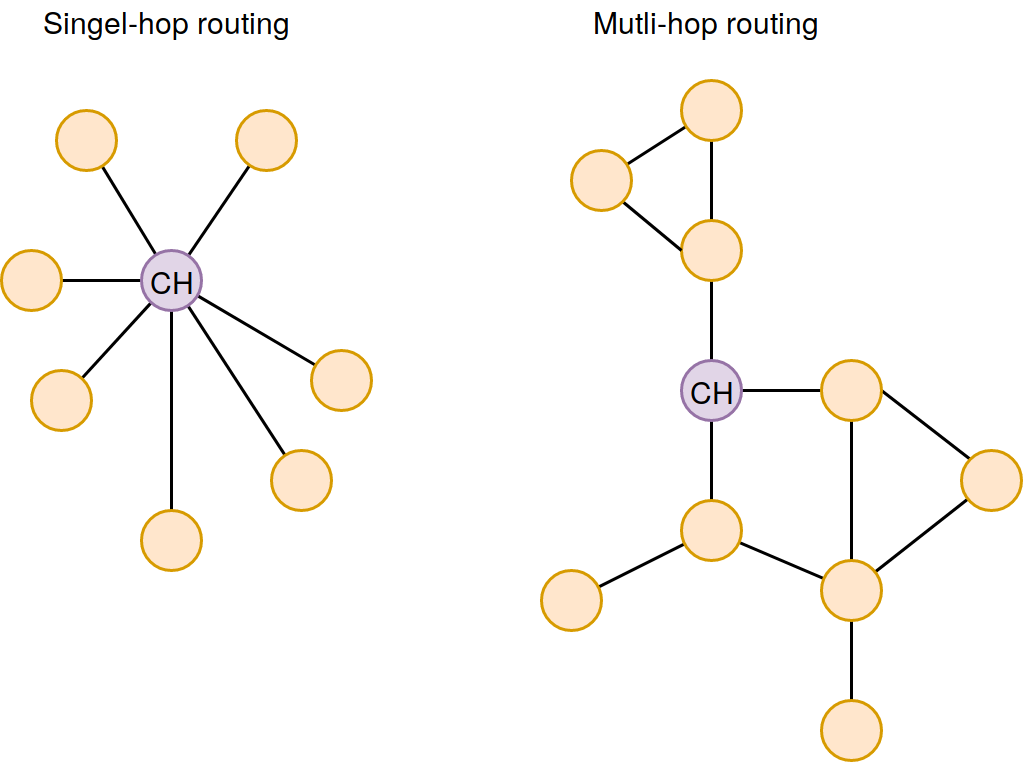
\includegraphics[scale=0.35]{hopping.png}
\caption{Figure show single-hop routing and multi-hop routing.}
\label{fig:hopping}
\end{figure}


\section{Data Accumulation} \label{disc:data_acc}
%How to gather data? Receive a GET-post from BS or someone else telling the CH to accumulate/gather data or gather data periodically? How does a BS send a GET-request to CH?? The CH could not be in range of the BS, so maybe send to a node in range and forward msg all the way to CH.. But again, what if some nodes are sleeping to save battery? The CH will then not receive the msg..

%\subsection{Data Accumulation}
%How much memory does a node have?  Have priorities on data such that data with high priority is stored longer or sent first.. Delete low poriority data if full memory..

%Vector clocks..

In the current approach, the \glspl{ch} are always the ones that initiate a request to the other nodes in the cluster for collecting data. This means that regular nodes can not decide that they want to send data to their \gls{ch}. Another approach would be that the node's sends their data when they have new data or when they have almost used up their memory capacity. However, if nodes have new data regularly, this approach would not be efficient in terms of energy consumption because other nodes in the routing path must be awake to transmit the data further to the \gls{ch}. There is reason to think that there is a possibility that the majority of the nodes in the clusters are awake most of their time instead of sleeping and saving battery. 


%\subsection{Different DAO Stores wants different data..}



\section{Replication Of Data} \label{disc:repl_data}
In the current approach will nodes only accumulate data that haven't been accumulated earlier. This approach will therefore have some degree of replication because a nodes data will be accumulated at the next node in the routing path.

It may take long time before a \gls{ch} gets access to a \gls{bs} or is contacted by a data mule that collects the data. Meanwhile, the \gls{ch} may fail or die due to battery limitations and all its accumulated data will be lost.

An approach to this problem is to only let nodes delete its data if the \gls{ch} have delivered all the data to a \gls{bs} or a data mule. Otherwise, the data is stored at each node.
Replication of node data is important if a node fails and we need to access the nodes data. However, replication of data also require more memory but sensor nodes have limited memory. In this case, there is a need for finding a degree of replica that can both be memory efficient and handling system failures.

Another approach is to have multiple \glspl{ch} that collects the same data. In this approach, nodes that are not \glspl{ch} can delete their data when they have sent their data to the \gls{ch} to minimize memory usage.


% Can use fingerprint to identify data..

%\section{Prioritization Of Data}
%Critical, non-ciritcal data?

\section{Concurrent CH Election And Data Accumulation} \label{disc:simult_el_acc}
The current approach provides an eventual consistency when electing a new \gls{ch} as mentioned before. This may raise some issues when a data gathering occurs when an election is ongoing due to rapidly change of \gls{ch}s and paths to \gls{ch} before all nodes have an consistent \gls{ch} election, as mentioned in Section \ref{sec:conc_events}.

%\textit{Forklar litt mer om fasene i \gls{leach} og mine, fra Section \ref{sec:conc_events}...}

\gls{leach} have have divided their sysem into different rounds, as described in Chapter \ref{chap:related_work}. To improve our approach, we could have implemented our system to be divided into rounds such as in \gls{leach}. Instead of having timers to stall the next phase, an improvement to our approach could be to have a status at each node saying if the node is going through a \gls{ch} election, if it accumulates data to the \gls{ch} or if it's just waiting for requests. In this way, when one status is true, e.g. a \gls{ch} election, can't a data accumulation happens.


%node have status= acc/LE.. if one, the other can not happen..?


%Eventual/weak consistency with leader election.. Gossiping with an ID to check if node receive the msg before or not.. Updating leader..


\section{Base Station Access} \label{disc:bs_acc}
%how to access bs/superOU, does some nodes have longer radio range, bigger antenna thant other, bw etc..? Is there one node in the system that only observe the network so a node can contact this node and get info about the system and know e.g. CH or neighbours, or if negihbours died etc..?
At the current approach, all nodes have the same broadcast range to reach nearby neighbours. This means that there is no node that have access to a \gls{bs}.

Another question is how nodes or \gls{ch} have contact with \glspl{bs}. As discussed in \autoref{disc:ch_election}, can a node be elected as \gls{ch} if it has access to a \gls{bs}, if there are any placed in the same area as the nodes. Another approach is to use a data mules to collect data from the \glspl{ch}.
One problem is how the \gls{ch} should be contacted since the \gls{bs} or data mule don't know who has the data in the cluster. One approach is that they know who the \glspl{ch} are, another approach is to let the \gls{bs} or data mule contact an arbitrary node and let the node alert the \gls{ch} that it should send it's data.

%\defintion{A data mule is a vehicle that physically carries a computer with storage between remote locations to create data communication links and to collect data.}


%\section{Scalability?}
%Note to self: scale with partially centralized network.. how about multiple \gls{ch} to load balance work and maybe shorter path for nodes to leaders..

%\section{CAP Theorem?}
%Note to self: evt bygge det litt inn i teksten..


%\section{Battery lifetime?}

%\section{Routing Challenges in WSNs}
%\begin{itemize}
%\item Node deployment
%\item Energy consumption without losing accuracy
%\item Data reporting method
%\item Node/link heterogeneity
%\item Fault tolerance
%\item Scalability
%\item Network dynamics
%\item Transmission media
%\item Connectivity
%\item Coverage
%\item Data aggregation
%\item Quality of service
%\end{itemize}



\chapter{Conclusion}
\glsresetall
In this thesis, we have implemented a prototype of a \gls{wsn} system where nodes observe and accumulate data from other nodes for further use. We describe a system where nodes discover each other through a broadcast range and together they form clusters. Each cluster elect  a \gls{ch} which is responsible for sending out a request for gather and accumulate data from the other nodes in the cluster. This \gls{ch} is rotating to save battery. Even though our approach works as intended, there is a need for improvements in how a \gls{ch} is elected and when a \gls{ch} should accumulate data.

Our experiments showed that the system have a stable CPU and memory usage. We can also see that the number of receiving packets of accumulated data is lower than sent packets with accumulated data which indicates that the nodes in the system accumulates data when intended to reduce traffic on the paths to the \glspl{ch}.


\chapter{Future Work}
\glsresetall
We will outline some of the areas that can be elaborated in future work. These include:

\begin{itemize}
\item \textbf{Availability of node}: In the current implementation can node join the cluster without any requirements, as discussed in \autoref{disc:node_conn}. We discuss how  how we could improve the implementation by having the \gls{ch} take the decision if a node can join the cluster or not. We also discussed how to improve a nodes knowledge about the network around them and how to get the newest information.

\item \textbf{\gls{ch} election:} The \gls{ch} election, together with the \gls{ch} calculation, in the current solution is not the best, but it is an introduction to a solution. As mentioned in \autoref{disc:ch_election}, would another approach be to include sub-factors such as power left on node, network traffic, number of neighbours etc, to calculate which nodes that are most qualified to be a \gls{ch}. 

\item \textbf{Multiple \glspl{ch}:} This implementation of the system does not support multiple \glspl{ch} in one cluster. In Section \autoref{disc:multi_ch}, we discuss how we could have improve our approach by to load balance work, possibly provide shorter paths for some nodes to \glspl{ch} and minimize scalability and performance issues.

\item \textbf{Access to \gls{bs}:} The current approach have no \gls{bs} or data mule to collect the data. In \autoref{disc:bs_acc}, we discuss how the cluster should get access to a \gls{ch} by implementing either a \gls{bs} or a data mule and how these should contact the nodes in the network.

%\item Approach for nodes observing other nodes..
\end{itemize}



\chapter{Appendix}
%Readme



\backmatter

%%% BIBLOGRAPHY

\newpage{}

\begin{thebibliography}{9}

%1
\bibitem{coat2016}
Åshild Ø. Pedersen, A. Stien, E. Soininen, and R. A. Ims,
\newblock {\em Climate-ecological observatory for arctic tundra-status 2016}, Mars 2016,
\newblock in {\em  Fram Forum 2016, pages 36-43.}
%\newblock {\em \url{http://www.framsenteret.no/getfile.php/2435814.1574.xyxruwywpp/FinalPDF_COAT.pdf}}.

%2
\bibitem{leach}
W. R. Heinzelman and A. Chandrakasan and H. Balakrishnan,
\newblock {\em Energy-efficient communication protocol for wireless microsensor networks}, 2000,
\newblock in {\em Proceedings of the 33rd Annual Hawaii International Conference on System Sciences, 10 pp. vol.2-}.

%3 - ikke printet ut
\bibitem{leach_perf}
K. Latif and M. Jaffar and N. Javaid and M. N. Saqib and U. Qasim and Z. A. Khan,
\newblock {\em Performance Analysis of Hierarchical Routing Protocols in Wireless Sensor Networks}, 2012,
\newblock in {\em 2012 Seventh International Conference on Broadband, Wireless Computing, Communication and Applications, pp. 620-625}.

%4 ikke i bruk
%\bibitem{fuzzy_rule}
%K. Gotefode and K. Kolhe,
%\newblock {\em Energy efficiency in wireless sensor network using Fuzzy rule and tree based routing protocol}, 2015,
%\newblock in {\em 2015 International Conference on Energy Systems and Applications, pp. 712-717}.

%5
\bibitem{tree_based}
Z. Han and J. Wu and J. Zhang and L. Liu and K. Tian,
\newblock {\em A General Self-Organized Tree-Based Energy-Balance Routing Protocol for Wireless Sensor Network}, 2014,
\newblock in {\em IEEE Transactions on Nuclear Science Vol.61, Nr.2, pp. 732-740}.

%6 ikke i bruk
\bibitem{routing_survey}
J. N. Al-Karaki and A. E. Kamal,
\newblock {\em Routing techniques in wireless sensor networks: a survey}, 2004,
\newblock in {\em IEEE Wireless Communications Vol.11, Nr.6, pp. 6-28}.

%7
\bibitem{pegasis}
S. Lindsey and C. S. Raghavendra,
\newblock {\em PEGASIS: Power-efficient gathering in sensor information systems}, 2002,
\newblock in {\em Proceedings, IEEE Aerospace Conference Vol.3, pp. 3-1125-3-1130}.

%8 - ikke skrevet ut/ ikke i bruk
%\bibitem{atyp_routing}
%X. Liu,
%\newblock {\em Atypical Hierarchical Routing Protocols for Wireless Sensor Networks: A Review}, 2015,
%\newblock in {\em IEEE Sensors Journal Vol.15, Nr.10, pp. 5372-5383}.

%9
\bibitem{fuzzy_logic}
A. K. Mishra and R. Kumar and J. Singh,
\newblock {\em A review on fuzzy logic based clustering algorithms for wireless sensor networks}, 2015,
\newblock in {\em 2015 International Conference on Futuristic Trends on Computational Analysis and Knowledge Management (ABLAZE), pp. 489-494}.

%10
\bibitem{ch_fuzzy}
Indranil Gupta and D. Riordan and Srinivas Sampalli,
\newblock {\em Cluster-head election using fuzzy logic for wireless sensor networks}, 2005,
\newblock in {\em 3rd Annual Communication Networks and Services Research Conference (CNSR'05), pp. 255-260}.

%11
\bibitem{dec_cb_alg}
Maryam Sabet and Hamid Reza Naji,
\newblock {\em A decentralized energy efficient hierarchical cluster-based routing algorithm for wireless sensor networks}, 2015,
\newblock in {\em AEU - International Journal of Electronics and Communications Vol.69, Nr.5, pp. 790 - 799}.

%12 ikke i bruk
%\bibitem{rout_prot_survey}
%Shio Kumar Singh, M P Singh and D K Singh,
%\newblock {\em Routing Protocols in Wireless Sensor Networks – A Survey }, 2010,
%\newblock in {\em International Journal of Computer Science \& Engineering Survey (IJCSES) Vol.1, No.2, November 2010, pp. 63-83}.

%13
\bibitem{leach_c}
W. B. Heinzelman and A. P. Chandrakasan and H. Balakrishnan,
\newblock {\em An application-specific protocol architecture for wireless microsensor networks},
\newblock in {\em IEEE Transactions on Wireless Communications Vol.1, No.4, October 2002, pp. 660-670}.

%14
\bibitem{demers}
Demers, Alan and Greene, Dan and Hauser, Carl and Irish, Wes and Larson, John and Shenker, Scott and Sturgis, Howard and Swinehart, Dan and Terry, Doug,
\newblock {\em Epidemic algorithms for replicated database maintenance},
\newblock in {\em ACM: Proceedings of the Sixth Annual ACM Symposium on Principles of Distributed Computing, 1987, pp. 1--12}.

%15
\bibitem{leach_e}
Chen, Bai and Zhang, Yaxiao and Li, Yuxian and Hao, Xiao-Chen and Fang, Yan,
\newblock {\em A Clustering Algorithm of Cluster-head Optimization for Wireless Sensor Networks Based on Energy},
\newblock in {\em Journal of Information and Computational Science, Vol.8, 2011}.

%16
\bibitem{leach_b}
M. Tong and M. Tang,
\newblock {\em LEACH-B: An Improved LEACH Protocol for Wireless Sensor Network},
\newblock in {\em J2010 6th International Conference on Wireless Communications Networking and Mobile Computing (WiCOM), 2010, pp. 1-4}.

%17 ikke i bruk
\bibitem{zebranet}
Juang, Philo and Oki, Hidekazu and Wang, Yong and Martonosi, Margaret and Peh, Li Shiuan and Rubenstein, Daniel,
\newblock {\em Energy-efficient Computing for Wildlife Tracking: Design Tradeoffs and Early Experiences with ZebraNet},
\newblock in {\em ACM: SIGARCH Comput. Archit. News, Vol.30, No.5, December 2002, pp. 96--107}.

%18 ikke i bruk
%\bibitem{dataColl}
%Di Francesco, Mario and Das, Sajal K. and Anastasi, Giuseppe,
%\newblock {\em Data Collection in Wireless Sensor Networks with Mobile Elements: A Survey},
%\newblock in {\em ACM Trans. Sen. Netw., Vol.8, No.1, August 2011, pp. 7:1--7:31}.

%19 ikke i bruk
\bibitem{gbsampling}
Jelasity, M\'{a}rk and Voulgaris, Spyros and Guerraoui, Rachid and Kermarrec, Anne-Marie and van Steen, Maarten,
\newblock {\em Gossip-based Peer Sampling},
\newblock in {\em ACM Trans. Comput. Syst., Vol.25, No.3, August 2007}.

%20 ikke i bruk
\bibitem{multiradio}
Draves, Richard and Padhye, Jitendra and Zill, Brian,
\newblock {\em Routing in Multi-radio, Multi-hop Wireless Mesh Networks},
\newblock in {\em Proceedings of the 10th Annual International Conference on Mobile Computing and Networking, 2004, pp.114--128}.

%21
\bibitem{wsnbook}
Holger Karl, Andreas Willig,
\newblock {\em Protocols and Architectures for Wireless Sensor Networks},
\newblock {John Wiley \& Sons, Ltd, 2006}.

%22
\bibitem{gaf}
Xu, Ya and Heidemann, John and Estrin, Deborah,
\newblock {\em Geography-informed Energy Conservation for Ad Hoc Routing},
\newblock in {\em MobiCom '01: Proceedings of the 7th Annual International Conference on Mobile Computing and Networking, 2001, pp.70--84}.

%23
\bibitem{gear}
Yu, Yan and Govindan, Ramesh and Estrin, Deborah,
\newblock {\em Geographical and Energy Aware Routing: a recursive data dissemination protocol for wireless sensor networks},
\newblock in {\em UCLA Computer Science Department Technical Report, Vol.463, 2001}.

%24
\bibitem{dsbook}
Tanenbaum, Andrew S. and Steen, Maarten van,
\newblock {\em Distributed Systems: Principles and Paradigms (2Nd Edition)},
\newblock {Prentice-Hall, Inc., 2014}.

%25
\bibitem{dijkstra}
Dijkstra, E. W.,
\newblock {\em A note on two problems in connexion with graphs},
\newblock in {\em Numerische Mathematik, Vol.1, No.1, December 1959, pp.269--271}.


%26
\bibitem{golangPsutil}
W. Shirou,
\newblock {\em gopsutil: psutil for golang},
\newblock in {\em GitHub: GitHub repository},
\newblock {\url{https://github.com/shirou/gopsutil}}, last commit={ \textit{57f370e}}.

%27
\bibitem{bully}
H. Garcia-Molina,
\newblock {\em Elections in a Distributed Computing System},
\newblock in {\em IEEE Transactions on Computers, 1982, Vol.C-31, No.1, pp.48-59}.

%28
\bibitem{euclidean}
H. Garcia-Molina,
\newblock {\em Euclidean space, ed. (2001)[1994]},
\newblock in {\em  Encyclopedia of Mathematics, Springer Science+Business Media B.V. / Kluwer Academic Publishers}.
\newblock {URL: \url{http://www.encyclopediaofmath.org/index.php?title=Euclidean_space&oldid=38673}}.

%29
\bibitem{dataAgg}
J. N. Al-Karaki and R. Ul-Mustafa and A. E. Kamal,
\newblock {\em Data aggregation in wireless sensor networks - exact and approximate algorithms},
\newblock in {\em  2004 Workshop on High Performance Switching and Routing, 2004. HPSR.}, pp.241-245.

%30
\bibitem{adfidelity}
Estrin, Deborah and Govindan, Ramesh and Heidemann, John and Kumar, Satish,
\newblock {\em Next Century Challenges: Scalable Coordination in Sensor Networks},
\newblock in {\em Proceedings of the 5th Annual ACM/IEEE International Conference on Mobile Computing and Networking}, 1999, pp.263--270.


%31
\bibitem{hopping2}
S. Fedor and M. Collier,
\newblock {\em On the Problem of Energy Efficiency of Multi-Hop vs One-Hop Routing in Wireless Sensor Networks},
\newblock in {\em Advanced Information Networking and Applications Workshops, 2007, AINAW '07. 21st International Conference on}, 2007, Vol.2, pp.380-385.


%31
\bibitem{dao}
O. Anshus,
\newblock {\em Distributed Arctic Observatory (DAO): A Cyber-Physical System for Ubiquitous Data and Services Covering the Arctic Tundra}, 2018
\newblock in {\url{https://www.forskningsradet.no/prognett-iktpluss/Nyheter/NOK_200_million_for_13_research_projects_on_Ubiquitous_data_and_services/1254032932215?lang=no}}, "Norwegian Research Council (NRC) - Project no: 270672"


\end{thebibliography}


\end{document}

